% $Id$
% 
%       This source code is part of
% 
%        G   R   O   M   A   C   S
% 
% GROningen MAchine for Chemical Simulations
% 
%               VERSION 2.0
% 
% Copyright (c) 1991-1999
% BIOSON Research Institute, Dept. of Biophysical Chemistry
% University of Groningen, The Netherlands
% 
% Please refer to:
% GROMACS: A message-passing parallel molecular dynamics implementation
% H.J.C. Berendsen, D. van der Spoel and R. van Drunen
% Comp. Phys. Comm. 91, 43-56 (1995)
% 
% Also check out our WWW page:
% http://md.chem.rug.nl/~gmx
% or e-mail to:
% gromacs@chem.rug.nl
% 
% And Hey:
% Gnomes, ROck Monsters And Chili Sauce
%

\chapter{Interaction function and force field\index{force-field}}
\label{ch:ff}
A force field is built up from two distinct components:
\begin{itemize}
\item The set of equations (called the {\em
\swapindex{potential}{function}s}) used to generate the potential
energies and their derivatives, the forces.
\item The parameters used in this set of equations
\end{itemize}
Within one set of equations various sets of parameters can be
used. Care must be taken that the combination of equations and
parameters form a consistent set. It is in general dangerous to make
{\em ad hoc} changes in a subset of parameters, because the various
contributions to the total force are usually interdependent.

{\gromacs} {\gmxver} includes several force fields, and additional ones
are available on the website. If you don't know which one to select
we recommend Gromos96 for united-atom setups and OPLS-AA/L for all-atom
parameters. The {\gromacs} forcefields is mainly included for historical
reasons; it is based on
\gromosv{87}~\cite{biomos}\index{gromos-87},
with a small modification concerning the interaction between
water-oxygens and carbon atoms~\cite{Buuren93b,Mark94}, as well as 10
extra atom types~\cite{Jorgensen83,Buuren93a,Buuren93b,Mark94,Liu95}.
However, the user is free to make her own modifications (beware!).
This will be explained in details in \chref{top}, which deals
with the {\bf Topology}. The organization of the force field files
is described in \secref{fforganization}.

To accommodate the potential functions used
in some popular force fields, {\gromacs} offers a choice of functions,
both for non-bonded interaction and for dihedral interactions. They
are described in the appropriate subsections.

The potential functions can be subdivided into three parts
\begin{enumerate}
\item   {\em Non-bonded}: Lennard-Jones or Buckingham, and Coulomb or
modified Coulomb. The non-bonded interactions are computed on the
basis of a neighbor list (a list of non-bonded atoms within a certain
radius), in which exclusions are already removed.
\item   {\em Bonded}: covalent bond-stretching, angle-bending,
improper dihedrals, and proper dihedrals. These are computed on the
basis of fixed lists. 
\item   {\em Restraints}: position restraints, angle restraints,
distance restraints, orientation restraints and dihedral restraints, all
based on fixed lists. 
\end{enumerate}

\section{Non-bonded interactions}
Non-bonded interactions in {\gromacs} are pair-additive and centro-symmetric:
\beq
V(\ve{r}_1,\ldots \ve{r}_N) = \sum_{i<j}V_{ij}(\rvij);
\eeq
\beq
\ve{F}_i = -\sum_j \frac{dV_{ij}(r_{ij})}{dr_{ij}} \frac{\rvij}{r_{ij}} = -\ve{F}_j
\eeq
The non-bonded interactions contain a \normindex{repulsion} term, 
a \normindex{dispersion}
term, and a Coulomb term. The repulsion and dispersion term are
combined in either the Lennard-Jones (or 6-12 interaction), or the
Buckingham (or exp-6 potential). In addition, (partially) charged atoms
act through the Coulomb term. 

\subsection{The Lennard-Jones interaction}
\label{sec:lj}
The \normindex{Lennard-Jones} potential $V_{LJ}$ between two atoms equals
\beq
V_{LJ}(\rij) =  \frac{C_{ij}^{(12)}}{\rij^{12}} -
                        \frac{C_{ij}^{(6)}}{\rij^6}     
\eeq
see also \figref{lj}
The parameters $C^{(12)}_{ij}$ and $C^{(6)}_{ij}$  depend on pairs of
{\em atom types}; consequently they are taken from a matrix of
LJ-parameters.

\begin{figure}
\centerline{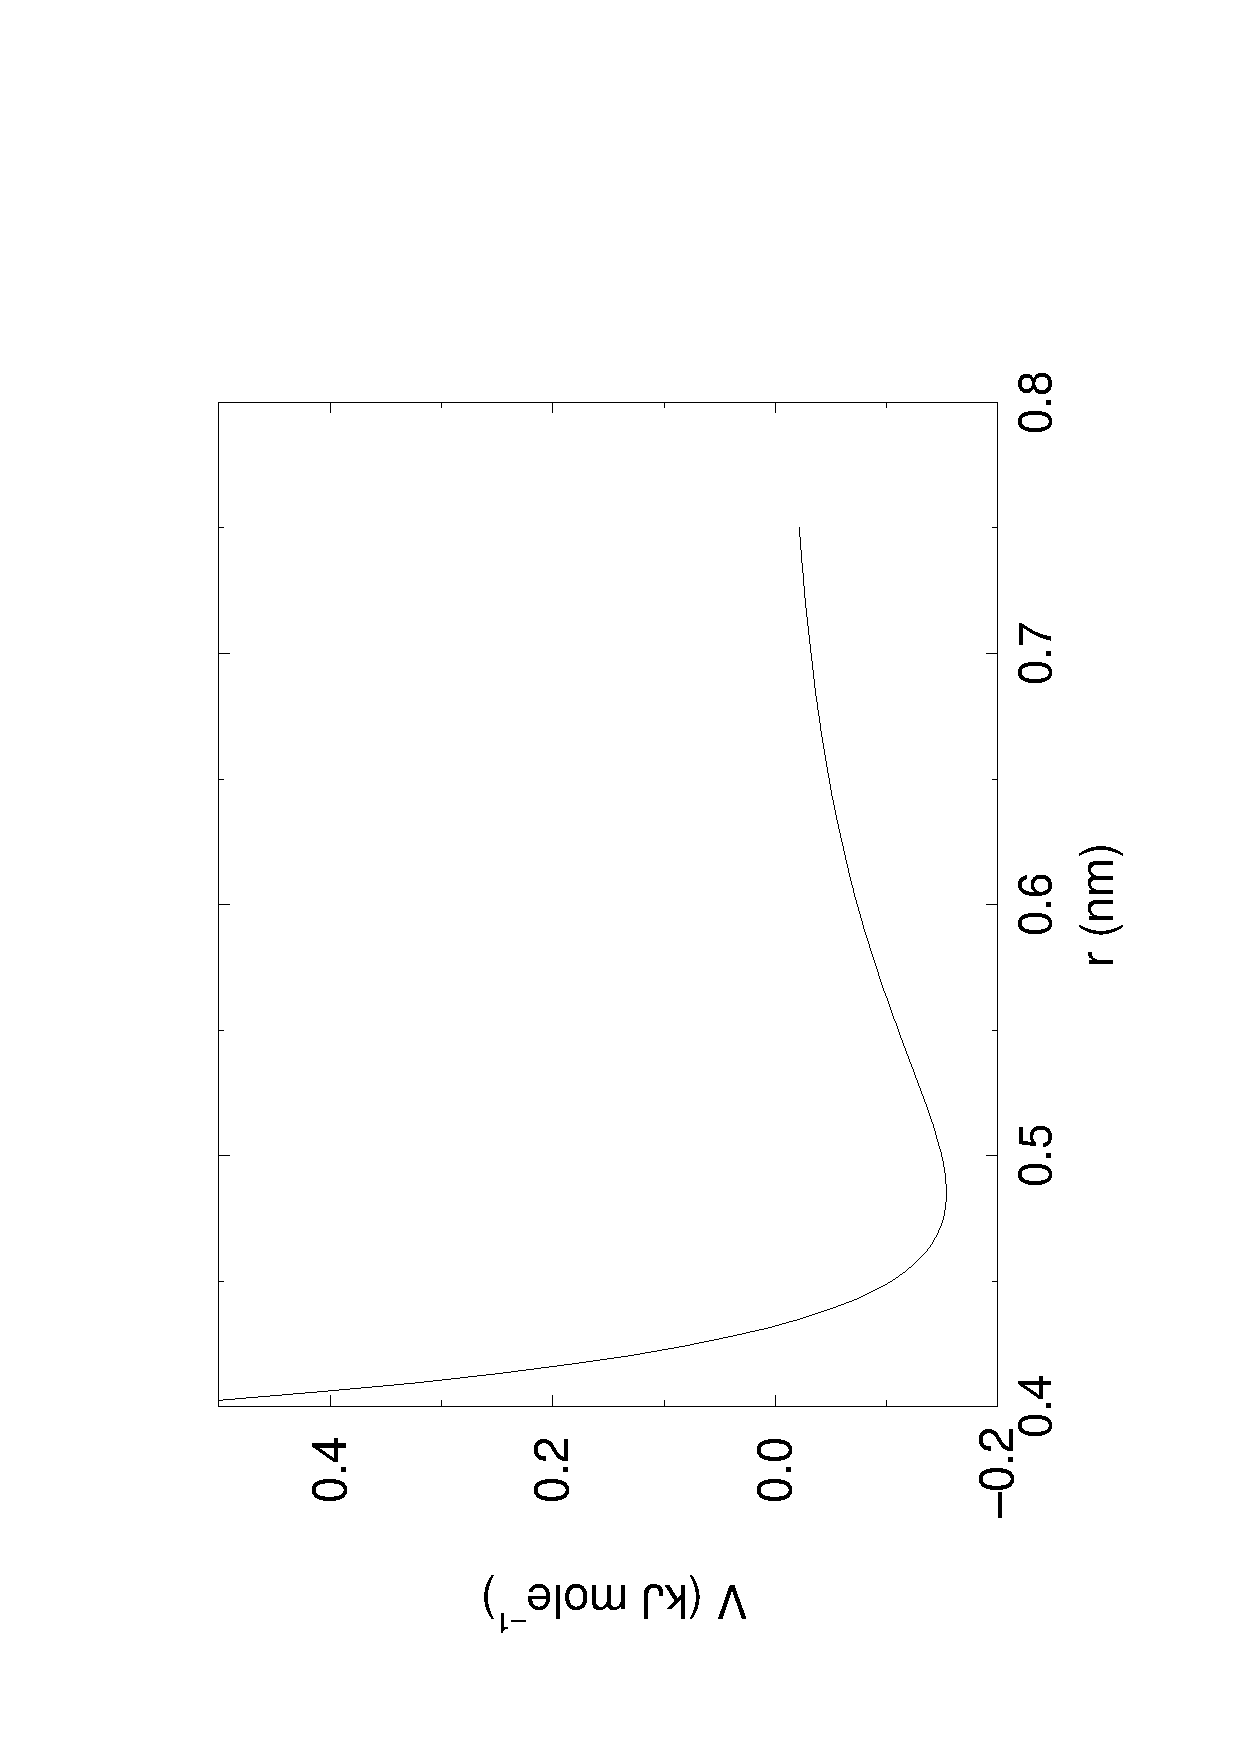
\includegraphics[angle=270,width=8cm]{plots/f_lj}}
\caption {The Lennard-Jones interaction.}
\label{fig:lj}
\end{figure}
 
The force derived from this potential is:
\beq
\ve{F}_i(\rvij) = \left( 12~\frac{C_{ij}^{(12)}}{\rij^{13}} -
                                 6~\frac{C_{ij}^{(6)}}{\rij^7} \right) \rnorm 
\eeq

The LJ potential may also be written in the following form :
\beq
V_{LJ}(\rvij) = 4\epsilon_{ij}\left(\left(\frac{\sigma_{ij}} {\rij}\right)^{12}
                - \left(\frac{\sigma_{ij}}{\rij}\right)^{6} \right)
\label{eqn:sigeps}      
\eeq

In constructing the parameter matrix for the non-bonded LJ-parameters,
two types of combination rules can be used within {\gromacs}: 
\beq
\begin{array}{rcl}
C_{ij}^{(6)}    &=& \left({C_{ii}^{(6)} * C_{jj}^{(6)}}\right)^{1/2}    \\
C_{ij}^{(12)}   &=& \left({C_{ii}^{(12)} * C_{jj}^{(12)}}\right)^{1/2}
\label{eqn:comb}
\end{array}
\eeq
or, alternatively the Lorentz-Bertelot rules can be used. An arithmetic average is used for the sigma's, while a geometric average is used for the epsilon's,
\beq
\begin{array}{rcl}
 \sigma_{ij}   &=& \frac{1}{ 2}(\sigma_{ii}+\sigma_{jj})        \\
 \epsilon_{ij} &=& \left({\epsilon_{ii} \epsilon_{jj}}\right)^{1/2}
\end{array}
\eeq

\subsection{Buckingham potential}
The \normindex{Buckingham} 
potential has a more flexible and realistic repulsion term
than the Lennard-Jones interaction, but is also more expensive to
compute. The potential form is:
\beq
V_{bh}(\rij) = A_{ij} \exp(-B_{ij} \rij) -
                        \frac{C_{ij}}{\rij^6}
\eeq
\begin{figure}
\centerline{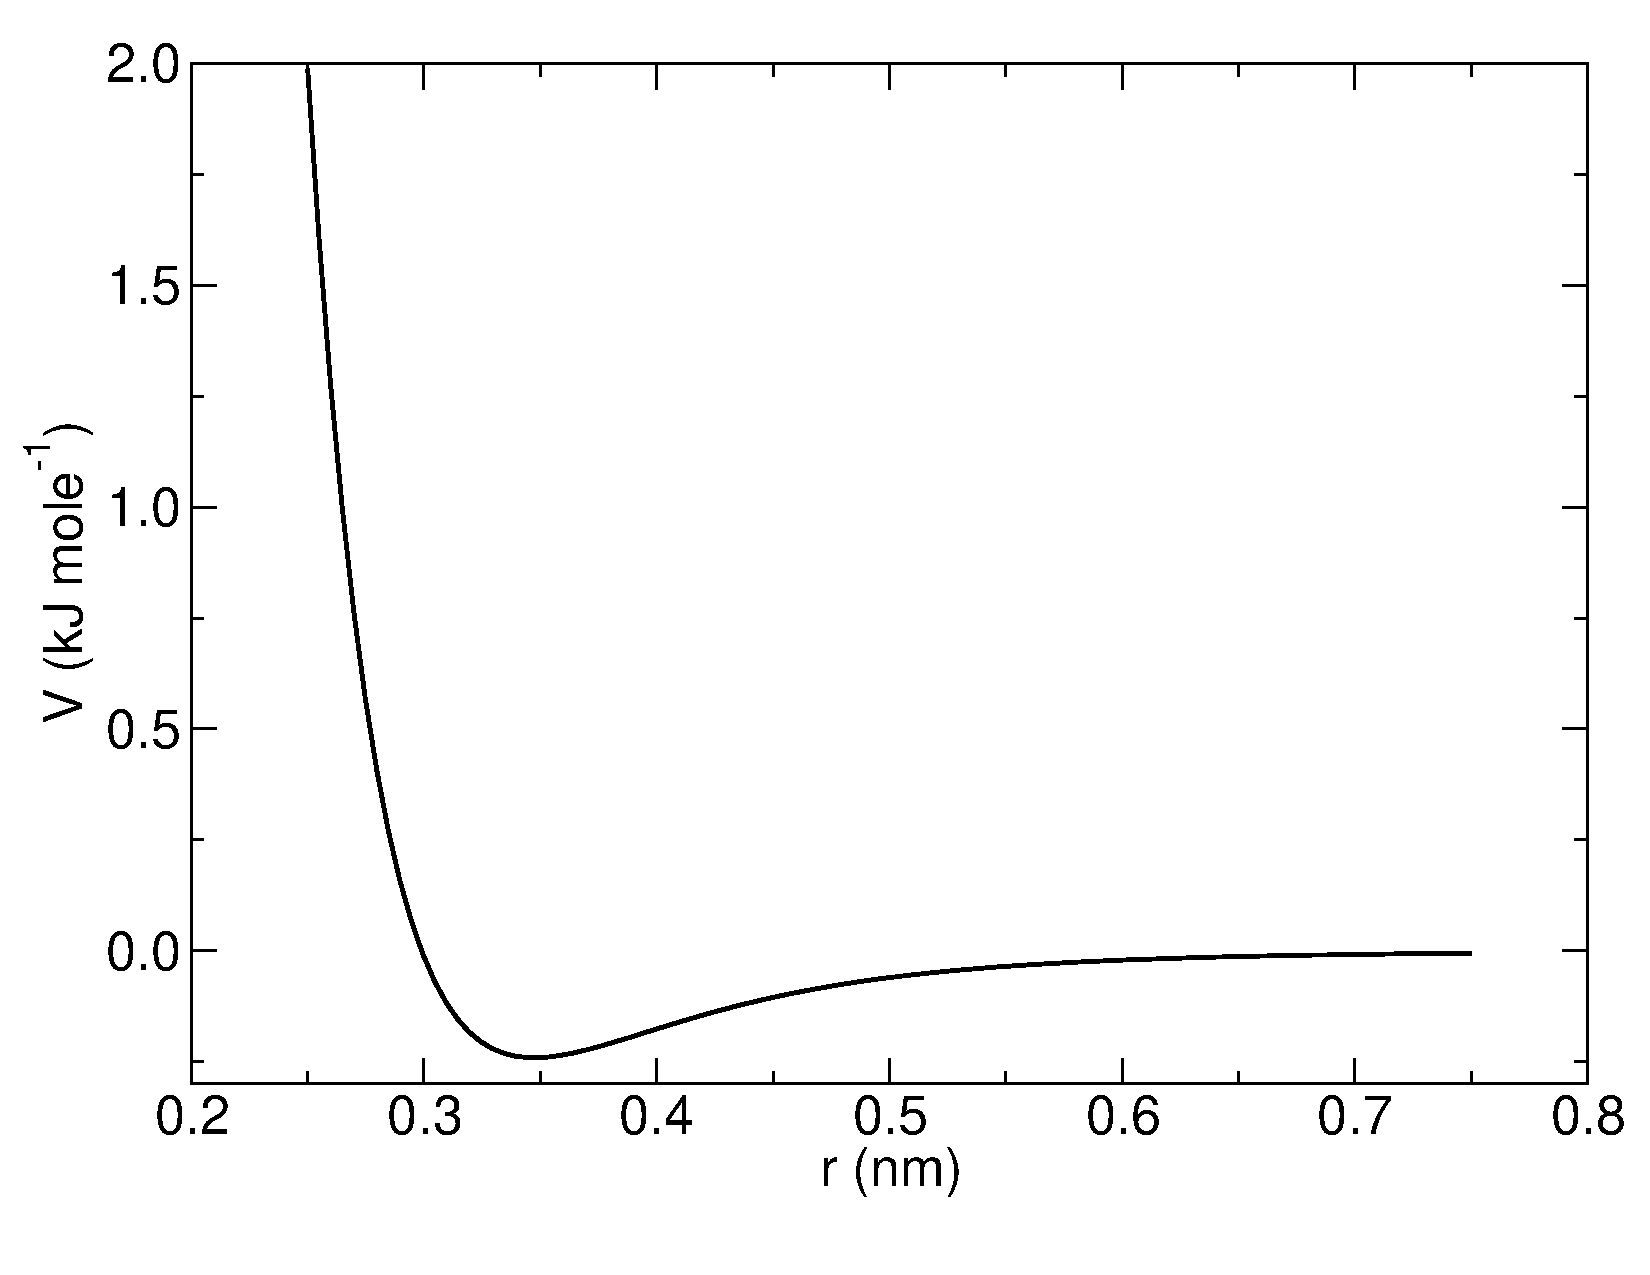
\includegraphics[angle=270,width=8cm]{plots/f_bham}}
\caption {The Buckingham interaction.}
\label{fig:bham}
\end{figure}

see also \figref{bham}, the force derived from this is:
\beq
 \ve{F}_i(\rij) = \left[ -A_{ij}B_{ij}\exp(-B_{ij} \rij) -
                                 6\frac{C_{ij}}{\rij^7} \right] \rnorm
\eeq

\subsection{Coulomb interaction}
\label{sec:coul}
\newcommand{\epsr}{\varepsilon_r}
\newcommand{\epsrf}{\varepsilon_{rf}}
The \normindex{Coulomb} interaction between two charge particles is given by:
\beq
V_c(\rij) = f \frac{q_i q_j}{\epsr \rij}
\label{eqn:vcoul}
\eeq
see also \figref{coul}, where $f = \frac{1}{4\pi \varepsilon_0} =
138.935\,485$ (see \chref{defunits})

\begin{figure}
\centerline{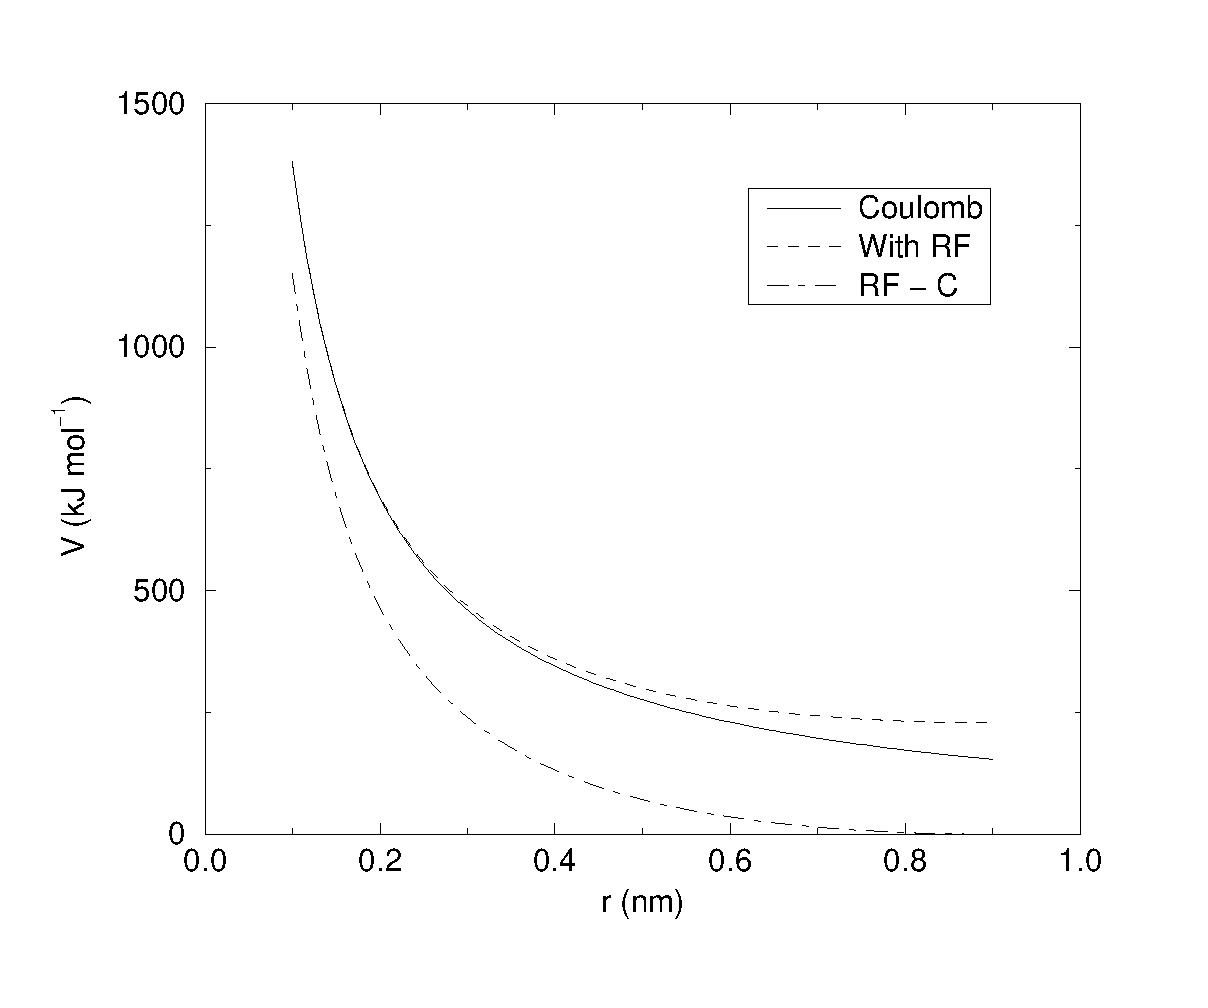
\includegraphics[width=8cm]{plots/vcrf}}
\caption[The Coulomb interaction with and without reaction field.]{The
Coulomb interaction (for particles with equal signed charge) with and
without reaction field. In the latter case $\epsr$ was 1, $\epsrf$ was 78,
and $r_c$ was 0.9 nm.
The dot-dashed line is the same as the dashed line, except for a constant.}
\label{fig:coul}
\end{figure}

The force derived from this potential is:
\beq
\ve{F}_i(\rvij) = f \frac{q_i q_j}{\epsr\rij^2}\rnorm
\eeq

In {\gromacs} the  relative \swapindex{dielectric}{constant} 
\normindex{$\epsr$}
may be set in the in the input for {\tt grompp}. 

\subsection{Coulomb interaction with \normindex{reaction field}}
\label{sec:coulrf}
The coulomb interaction can be modified for homogeneous systems, by
assuming a constant dielectric environment beyond the cutoff $r_c$
with a dielectric constant of {$\epsrf$}. The interaction then reads:
\beq
V_{crf} ~=~
  f \frac{q_i q_j}{\epsr\rij}\left[1+\frac{\epsrf-\epsr}{2\epsrf+\epsr}
  \,\frac{\rij^3}{r_c^3}\right]
  - f\frac{q_i q_j}{\epsr r_c}\,\frac{3\epsrf}{2\epsrf+\epsr}
\label{eqn:vcrf}
\eeq
in which the constant expression on the right makes the potential
zero at the cutoff $r_c$. For charged cut-off spheres this corresponds
to neutralization with a homogeneous background charge.
We can rewrite \eqnref{vcrf} for simplicity as
\beq
V_{crf} ~=~     f \frac{q_i q_j}{\epsr}\left[\frac{1}{\rij} + k_{rf}~ \rij^2 -c_{rf}\right]
\eeq
with
\bea
k_{rf}  &=&     \frac{1}{r_c^3}\,\frac{\epsrf-\epsr}{(2\epsrf+\epsr)}   \label{eqn:krf}\\
c_{rf}  &=&     \frac{1}{r_c}+k_{rf}\,r_c^2 ~=~ \frac{1}{r_c}\,\frac{3\epsrf}{(2\epsrf+\epsr)}
\label{eqn:crf}
\eea
For large $\epsrf$ the $k_{rf}$ goes to $r_c^{-3}/2$,
while for $\epsrf$ = $\epsr$ the correction vanishes.
In \figref{coul}
the modified interaction is plotted, and it is clear that the derivative 
with respect to $\rij$ (= -force) goes to zero at the cutoff distance.
The force derived from this potential reads:
\beq
\ve{F}_i(\rvij) = f \frac{q_i q_j}{\epsr}\left[\frac{1}{\rij^2} - 2 k_{rf}\rij\right]\rnorm
\label{eqn:fcrf}
\eeq
The reaction-field correction should also be applied to all excluded
atoms pairs, including self pairs, in which case the normal Coulomb
term in \eqnsref{vcrf}{fcrf} is absent.

Tironi {\etal} have introduced a generalized reaction field in which
the dielectric continuum beyond the cutoff $r_c$ also has an ionic strength
$I$~\cite{Tironi95}. In this case we can rewrite the constants $k_{rf}$ and 
$c_{rf}$ using the inverse Debye screening length $\kappa$:
\bea
\kappa^2  &=&     
   \frac{2 I \,F^2}{\varepsilon_0 \epsrf RT}
   = \frac{F^2}{\varepsilon_0 \epsrf RT}\sum_{i=1}^{K} c_i z_i     \\
k_{rf}  &=&     \frac{1}{r_c^3}\,
    \frac{(\epsrf-\epsr)(1 + \kappa r_c) + \half\epsrf(\kappa r_c)^2}
         {(2\epsrf + \epsr)(1 + \kappa r_c) + \epsrf(\kappa r_c)^2}
    \label{eqn:kgrf}\\
c_{rf}  &=&     \frac{1}{r_c}\,
    \frac{3\epsrf(1 + \kappa r_c + \half(\kappa r_c)^2)}
         {(2\epsrf+\epsr)(1 + \kappa r_c) + \epsrf(\kappa r_c)^2}
    \label{eqn:cgrf}
\eea
where $F$ is Faraday's constant, $R$ is the ideal gas constant, $T$
the absolute temperature, $c_i$ the molar concentration for species
$i$ and $z_i$ the charge number of species $i$ where we have $K$
different species. In the limit of zero ionic strength ($\kappa=0$)
\eqnsref{kgrf}{cgrf} reduce to the simple forms of \eqnsref{krf}{crf}
respectively.

\subsection{Modified non-bonded interactions}
In the {\gromacs} force field the non-bonded potentials can be
modified by a shift function. The purpose of this is to replace the
truncated forces by forces that are continuous and have continuous
derivatives at the \normindex{cutoff} radius. With such forces the
time-step integration produces much smaller errors and there are no
such complications as creating charges from dipoles by the truncation
procedure. In fact, by using shifted forces there is no need for
charge groups in the construction of neighbor lists. However, the
shift function produces a considerable modification of the Coulomb
potential. Unless the 'missing' long-range potential is properly
calculated and added (through the use of PPPM, Ewald, or PME), the
effect of such modifications must be carefully evaluated.  The
modification of the Lennard-Jones dispersion and repulsion is only
minor, but it does remove the noise caused by cutoff effects.
 
There is {\em no} fundamental difference between a switch function
(which multiplies the potential with a function) and a shift function
(which adds a function to the force or potential). The switch
function is a special case of the shift function, which we apply to
the {\em force function} $F(r)$, related to the electrostatic or
Van der Waals force acting on particle $i$ by particle $j$ as
\beq
\ve{F}_i = c F(r_{ij}) \frac{\rvij}{r_{ij}}
\eeq
For pure Coulomb or Lennard-Jones interactions
$F(r)=F_\alpha(r)=r^{-(\alpha+1)}$.
The shifted force $F_s(r)$ can generally be written as:
\beq
\begin{array}{rcl}
\vspace{2mm}
F_s(r)~=&~F_\alpha(r)   & r < r_1               \\
\vspace{2mm}
F_s(r)~=&~F_\alpha(r)+S(r)      & r_1 \le r < r_c       \\
F_s(r)~=&~0             & r_c \le r     
\end{array}
\eeq
When $r_1=0$ this is a traditional shift function, otherwise it acts as a 
switch function. The corresponding shifted coulomb potential then reads:
\beq
V_s(r_{ij}) = f \Phi_s (r_{ij}) q_i q_j
\eeq
where $\Phi(r)$ is the potential function 
\beq
\Phi_s(r) =  \int^{\infty}_r~F_s(x)\, dx
\eeq

The {\gromacs} shift function should be smooth at the boundaries, therefore
the following boundary conditions are imposed on the shift function:
\beq
\begin{array}{rcl}
S(r_1)          &=&0            \\
S'(r_1)         &=&0            \\
S(r_c)          &=&-F_\alpha(r_c)       \\
S'(r_c)         &=&-F_\alpha'(r_c)
\end{array}
\eeq
A 3$^{rd}$ degree polynomial of the form
\beq
S(r) = A(r-r_1)^2 + B(r-r_1)^3
\eeq
fulfills these requirements. The constants A and B are given by the
boundary condition at $r_c$: 
\beq
\begin{array}{rcl}
\vspace{2mm}
A &~=~& -\displaystyle
        \frac{(\alpha+4)r_c~-~(\alpha+1)r_1} {r_c^{\alpha+2}~(r_c-r_1)^2} \\
B &~=~& \displaystyle
        \frac{(\alpha+3)r_c~-~(\alpha+1)r_1}{r_c^{\alpha+2}~(r_c-r_1)^3}
\end{array}
\eeq
Thus the total force function is
\beq
F_s(r) = \frac{1}{r^{\alpha+1}} + A(r-r_1)^2 + B(r-r_1)^3
\eeq
and the potential function reads
\beq
\Phi(r) = \frac{1}{r^\alpha} - \frac{A}{3} (r-r_1)^3 - \frac{B}{4} (r-r_1)^4 - C
\eeq
where 
\beq
C =  \frac{1}{r_c^\alpha} - \frac{A}{3} (r_c-r_1)^3 - \frac{B}{4} (r_c-r_1)^4
\eeq

When $r_1$ = 0, the modified Coulomb force function is
\beq
 F_s(r) = \frac{1}{r^2} - \frac{5 r^2}{r_c^4} + \frac{4 r^3}{r_c^5}
\eeq
identical to the {\em \swapindex{parabolic}{force}} 
function recommended to be used as a short-range function in 
conjunction with a \swapindex{Poisson}{solver} 
for the long-range part~\cite{Berendsen93a}.
The modified Coulomb potential function is
\beq
\Phi(r) = \frac{1}{r} - \frac{5}{3r_c} + \frac{5r^3}{3r_c^4} - \frac{r^4}{r_c^5}
\eeq
see also \figref{shift}.

\begin{figure}
\centerline{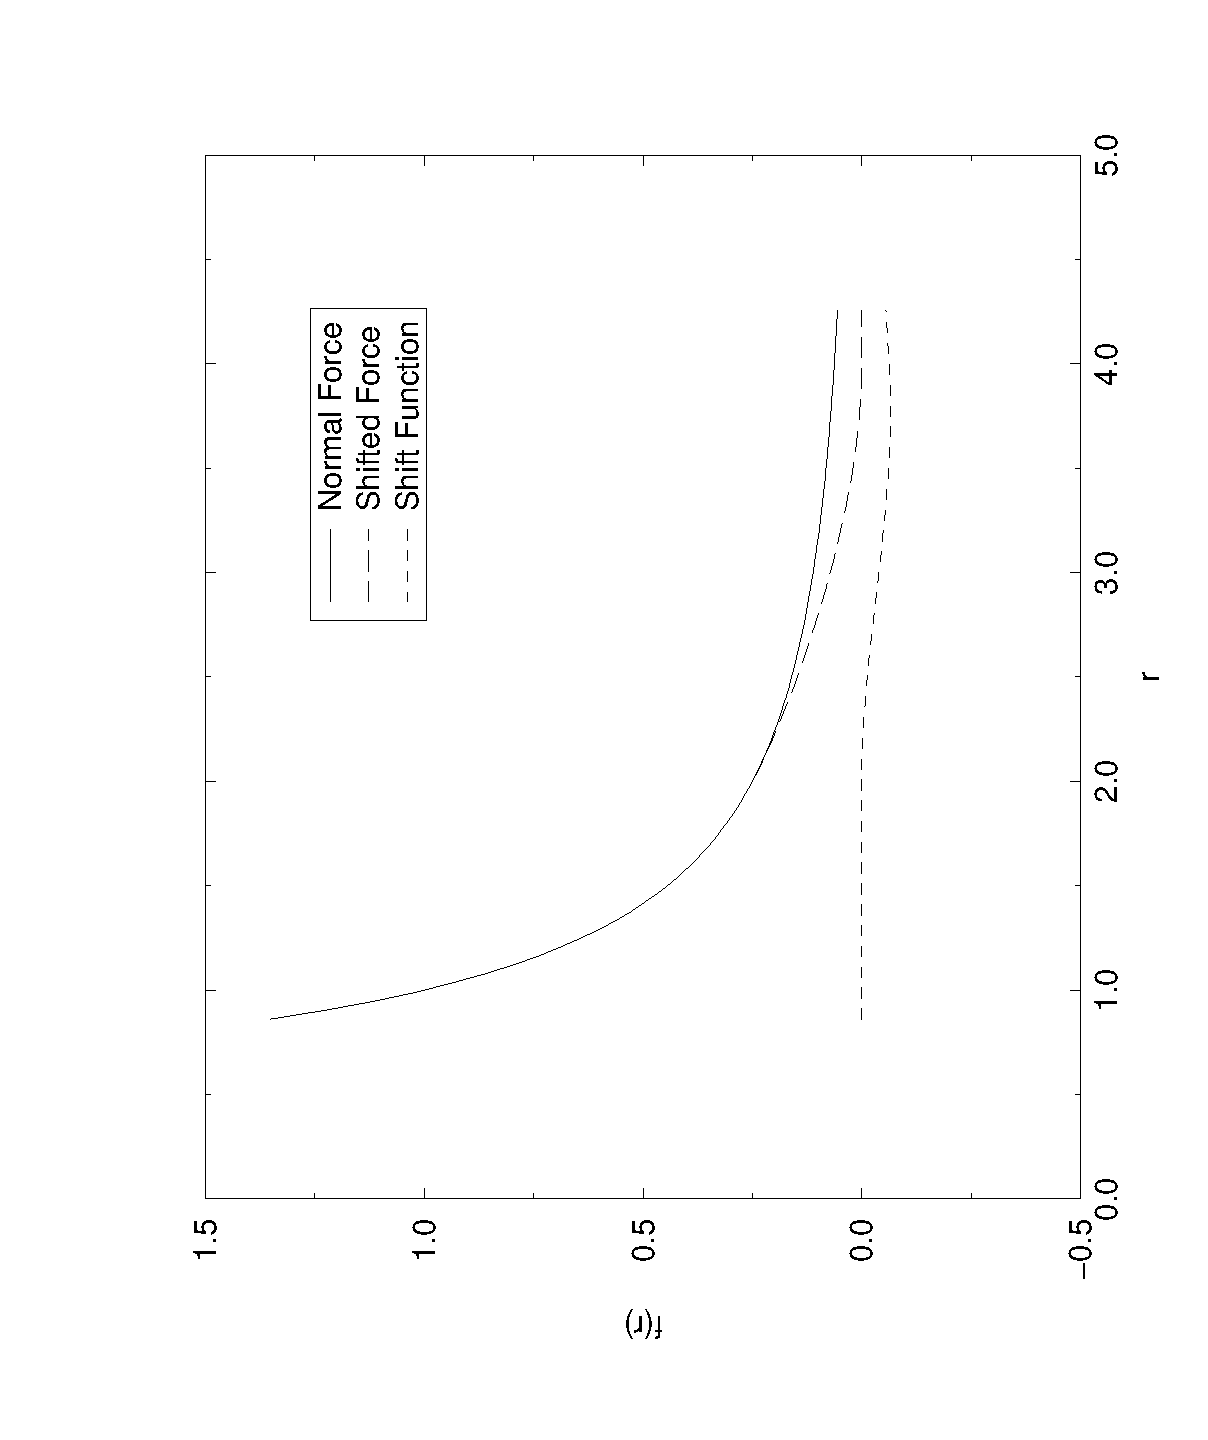
\includegraphics[angle=270,width=10cm]{plots/shiftf}}
\caption[The Coulomb Force, Shifted Force and Shift Function
$S(r)$,.]{The Coulomb Force, Shifted Force and Shift Function $S(r)$,
using r$_1$ = 2 and r$_c$ = 4.} 
\label{fig:shift}
\end{figure}

\subsection{Modified short-range interactions with Ewald summation}
When \normindex{Ewald sum}mation or \seeindex{particle-mesh
Ewald}{PME}\index{Ewald, particle-mesh} is used to calculate the
long-range interactions, the 
short-range coulomb potential must also be modified, similar to the
switch function above. In this case the short range potential is given
by
\beq
V(r) = f \frac{\mbox{erfc}(\beta r_{ij})}{r_{ij}} q_i q_j,
\eeq
where $\beta$ is a parameter that determines the relative weight 
between the direct space sum and the reciprocal space sum and erfc$(x)$ is
the complementary error function. For further 
details on long-range electrostatics, see \secref{lr_elstat}.


\section{Bonded interactions}
Bonded interactions are based on a fixed list of atoms. They are not
exclusively pair interactions, but include 3- and 4-body interactions
as well. There are {\em bond stretching} (2-body), {\em bond angle}
(3-body), and {\em dihedral angle} (4-body) interactions. A special
type of dihedral interaction (called {\em improper dihedral}) is used
to force atoms to remain in a plane or to prevent transition to a
configuration of opposite chirality (a mirror image).

\subsection{Bond stretching}
\label{sec:bondpot}
\subsubsection{Harmonic potential}
The \swapindex{bond}{stretching} between two covalently bonded atoms
$i$ and $j$ is represented by a harmonic potential

\begin{figure}
\centerline{\raisebox{-1.8cm}{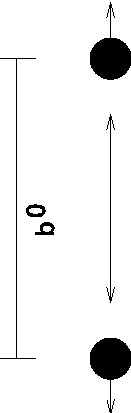
\includegraphics[angle=270,width=5cm]{plots/bstretch}}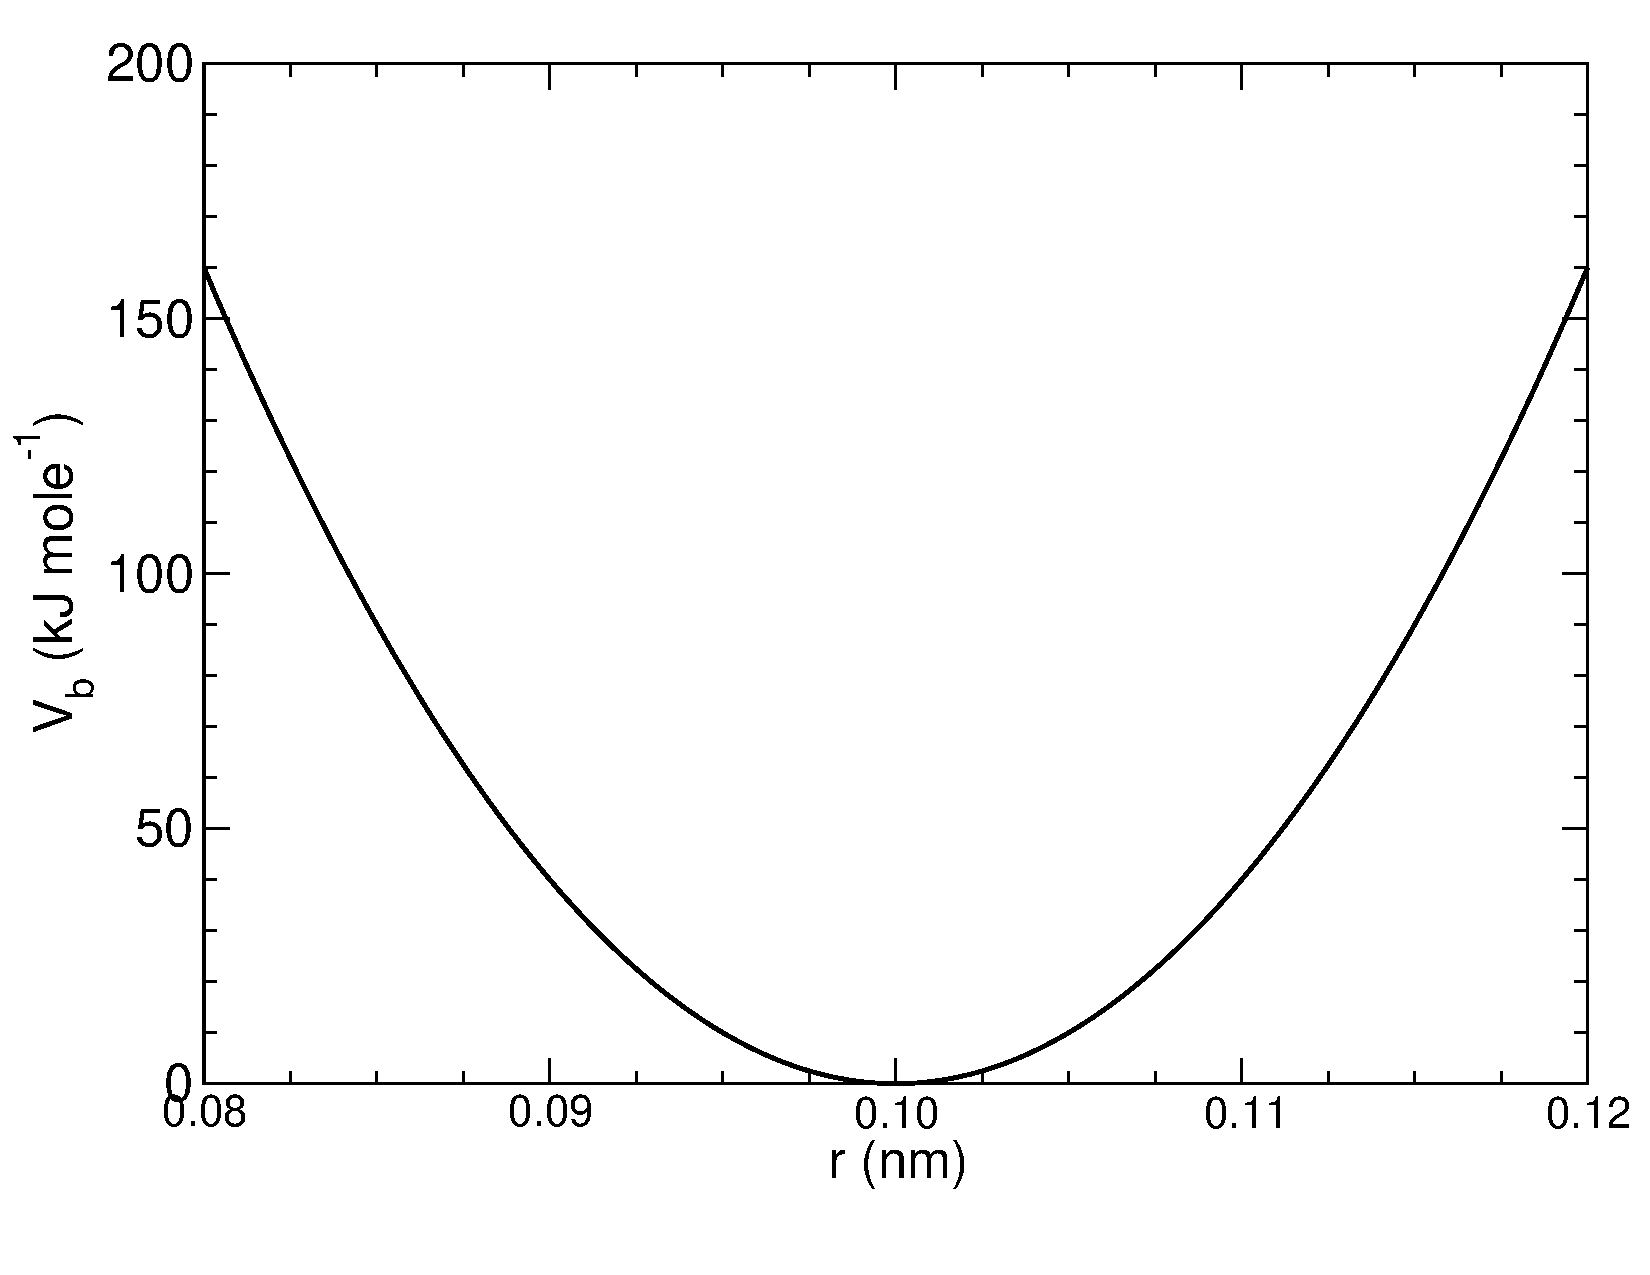
\includegraphics[angle=270,width=7cm]{plots/f_bond}}
\caption[Bond stretching.]{Principle of bond stretching (left), and the bond
stretching potential (right).}
\label{fig:bstretch1}
\end{figure}

\beq
V_b~(\rij) = \half k^b_{ij}(\rij-b_{ij})^2
\eeq
see also \figref{bstretch1}, with the force
\beq
\ve{F}_i(\rvij) = k^b_{ij}(\rij-b_{ij}) \rnorm
\eeq

\subsubsection{Fourth power potential}
In the \gromosv{96} force field~\cite{gromos96} the covalent bond potential
is written for reasons of computational efficiency as:
\beq
V_b~(\rij) = \frac{1}{4}k^b_{ij}\left(\rij^2-b_{ij}^2\right)^2
\eeq
the corresponding  force is:
\beq
\ve{F}_i(\rvij) = k^b_{ij}(\rij^2-b_{ij}^2)~\rvij
\eeq
The force constants for this form of the potential is related to the usual
harmonic force constant $k^{b,harm}$ (\secref{bondpot}) as
\beq
2 k^b b_{ij}^2 = k^{b,harm}
\eeq
The force constants are mostly derived from the harmonic ones used in 
\gromosv{87}~\cite{biomos}. Although this form is computationally more 
efficient
(because no square root has to be evaluated), it is conceptually more
complex. One particular disadvantage is that since the form is not harmonic,
the average energy of a single bond is not equal to $\half kT$ as it is for 
the normal harmonic potential.

\subsection{Morse potential bond stretching}
%\author{F.P.X. Everdij}
%
For some systems that require an anharmonic bond stretching potential,
the Morse potential~\cite{Morse29} 
between two atoms {\it i} and {\it j} is available
in {\gromacs}. This potential differs from the harmonic potential in
having an asymmetric potential well and a zero force at infinite
distance. The functional form is:
\beq
\displaystyle V_{morse} (r_{ij}) = D_{ij} [1 - \exp(-\beta_{ij}(r_{ij}-b_{ij}))]^2,
\eeq
see also \figref{morse}, and the corresponding force is:
\beq
\begin{array}{rcl}
\displaystyle {\bf F}_{morse} ({\bf r}_{ij})&=&2 D_{ij} \beta_{ij} r_{ij} \exp(-\beta_{ij}(r_{ij}-b_{ij})) * \\
\displaystyle \: & \: &[1 - \exp(-\beta_{ij}(r_{ij}-b_{ij}))] \frac{\displaystyle {\bf r}_{ij}}{\displaystyle r_{ij}},
\end{array}
\eeq
where \( \displaystyle D_{ij} \) is the depth of the well in kJ/mol,
\( \displaystyle \beta_{ij} \) defines the steepness of the well (in
nm\(^{-1} \)), and \( \displaystyle b_{ij} \) is the equilibrium
distance in nm.  The steepness parameter \( \displaystyle \beta_{ij}
\) can be expressed in terms of the reduced mass of the atoms {\it i}
and {\it j}, the fundamental vibration frequency \( \displaystyle
\omega_{ij} \) and the well depth \( \displaystyle D_{ij} \):
\beq
\displaystyle \beta_{ij}= \omega_{ij} \sqrt{\frac{\mu_{ij}}{2 D_{ij}}}
\eeq
and because \( \displaystyle \omega = \sqrt{k/\mu} \), one can rewrite \( \displaystyle \beta_{ij} \) in terms of the harmonic force constant \( \displaystyle k_{ij} \)
\beq
\displaystyle \beta_{ij}= \sqrt{\frac{k_{ij}}{2 D_{ij}}}
\label{eqn:betaij}
\eeq
For small deviations \( \displaystyle (r_{ij}-b_{ij}) \), one can
approximate the \( \displaystyle \exp \)-term to first-order using a
Taylor expansion:
\beq
\displaystyle \exp(-x) \approx 1-x
\label{eqn:expminx}
\eeq
and substituting \eqnref{betaij} and \eqnref{expminx} in the functional from,
\beq
\begin{array}{rcl}
\displaystyle V_{morse} (r_{ij})&=&D_{ij} [1 - \exp(-\beta_{ij}(r_{ij}-b_{ij}))]^2\\
\displaystyle \:&=&D_{ij} [1 - (1 -\sqrt{\frac{k_{ij}}{2 D_{ij}}}(r_{ij}-b_{ij}))]^2\\
\displaystyle \:&=&\frac{1}{2} k_{ij} (r_{ij}-b_{ij}))^2,
\end{array}
\eeq
we recover the harmonic bond stretching potential.

\begin{figure}
\centerline{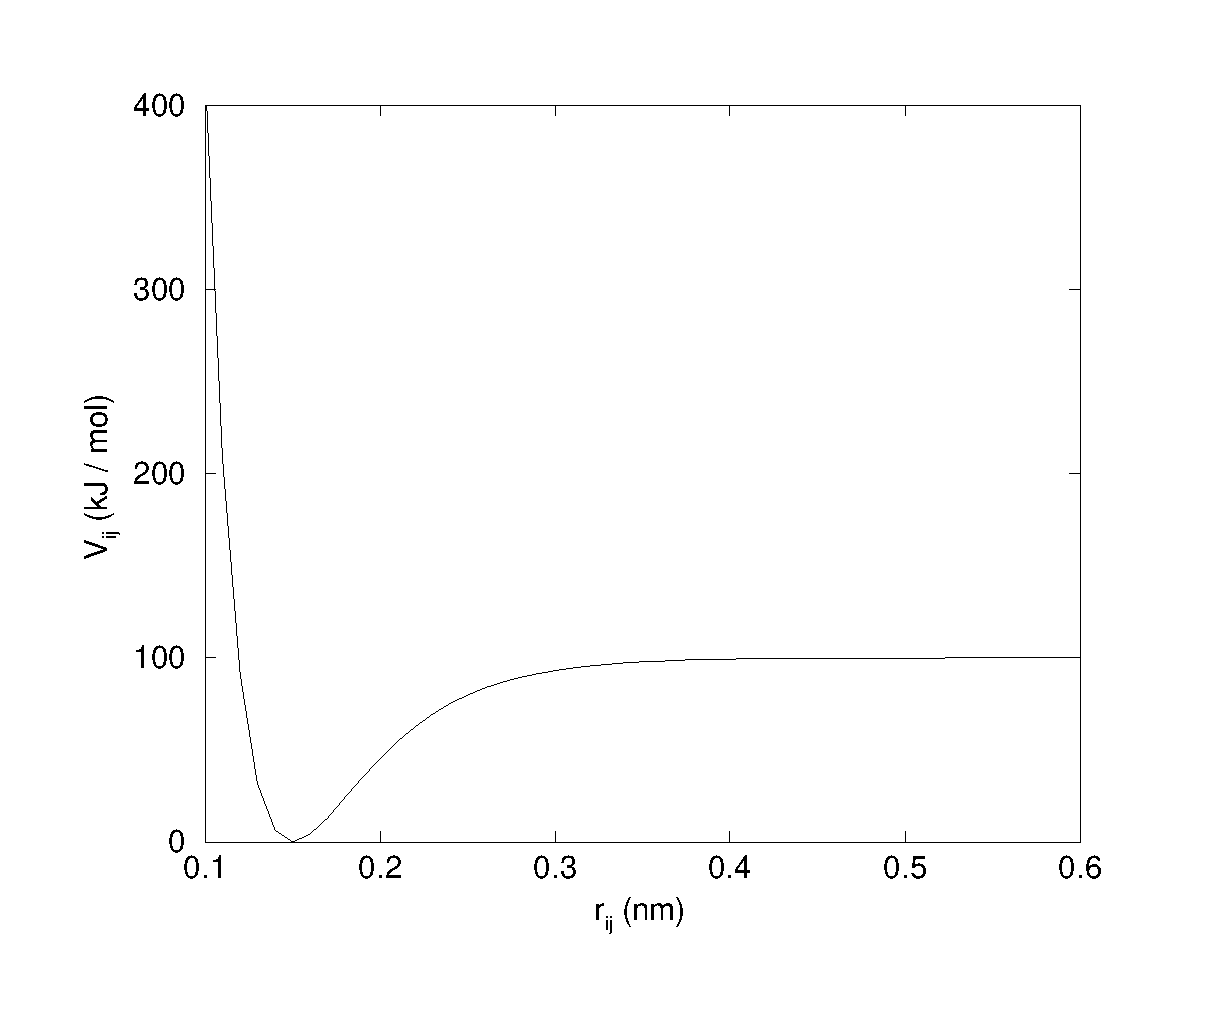
\includegraphics[width=7cm]{plots/f_morse}}
\caption{The Morse potential well, with bond length 0.15 nm.}
\label{fig:morse}
\end{figure}

\subsection{Cubic bond stretching potential}
Another anharmonic bond stretching potential that is slightly simpler
than the Morse potential adds a cubic term in the distance to the
simple harmonic form:
\beq
V_b~(\rij) = k^b_{ij}(\rij-b_{ij})^2 + k^b_{ij}k^{cub}_{ij}(\rij-b_{ij})^3
\eeq
A flexible \normindex{water} model (based on
the SPC water model~\cite{Berendsen81}) including 
a cubic bond stretching potential for the O-H bond
was developed by Ferguson~\cite{Ferguson95}. This model was found
to yield a reasonable infrared spectrum. The Ferguson water model is
available in the {\gromacs} library. 
It should be noted that the potential is asymmetric: overstretching leads to
infinitely low energies. The \swapindex{integration}{timestep} is therefore
limited to 1 fs.

The force corresponding to this potential is:
\beq
\ve{F}_i(\rvij) = 2k^b_{ij}(\rij-b_{ij})~\rnorm + 3k^b_{ij}k^{cub}_{ij}(\rij-b_{ij})^2~\rnorm
\eeq

\subsection{FENE bond stretching potential}
\index{FENE potential}
In coarse-grained polymer simulations the beads are often connected
by a FENE (finitely extendible nonlinear elastic) potential~\cite{Warner72}:
\beq
V_{\mbox{\small FENE}}(\rij) =
  -\half k^b_{ij} b^2_{ij} \log\left(1 - \frac{\rij^2}{b^2_{ij}}\right)
\eeq
The potential looks complicated, but the expression for the force is simpler:
\beq
F_{\mbox{\small FENE}}(\rvij) =
  k^b_{ij} \left(1 - \frac{\rij^2}{b^2_{ij}}\right)^{-1} \rvij
\eeq
At short distances the potential asymptotically goes to a harmonic
potential with force constant $k^b$, while it diverges at distance $b$.

\subsection{Harmonic angle potential}
\label{sec:anglepot}
\newcommand{\tijk}{\theta_{ijk}}
The bond \swapindex{angle}{vibration} between a triplet of atoms $i$ - $j$ - $k$
is also represented by a harmonic potential on the angle $\tijk$

\begin{figure}
\centerline{\raisebox{-1.5cm}{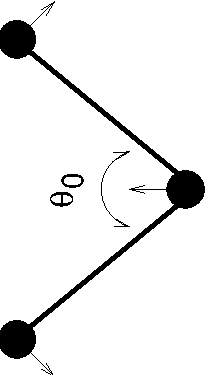
\includegraphics[angle=270,width=5cm]{plots/angle}}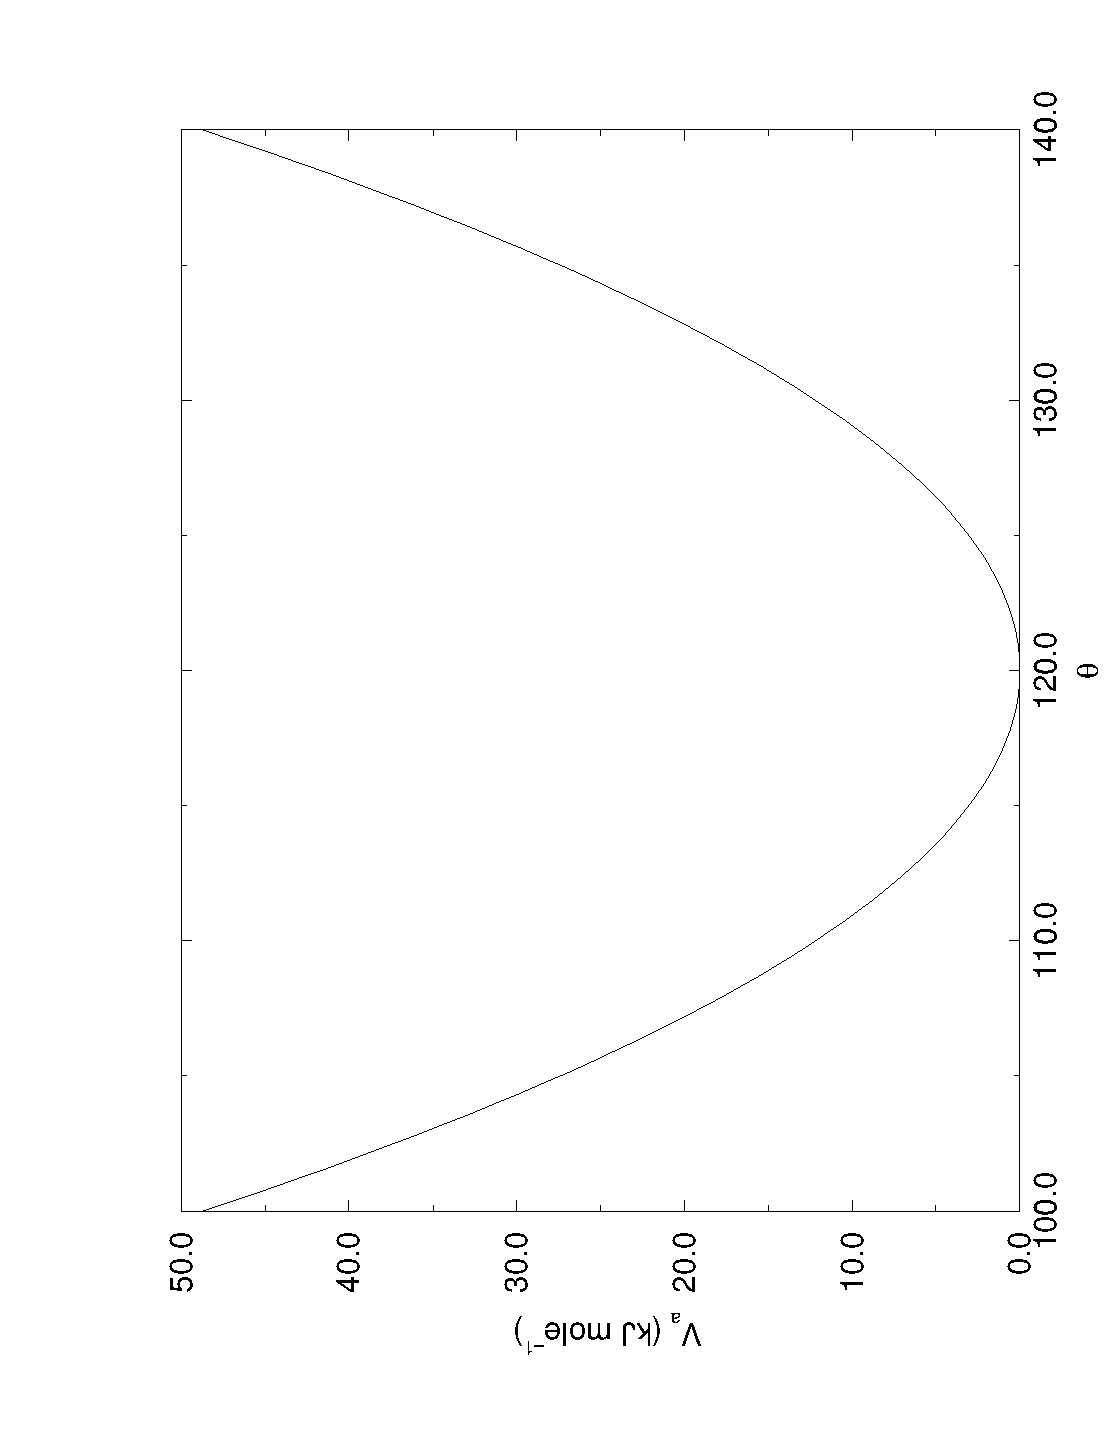
\includegraphics[angle=270,width=7cm]{plots/f_angle}}
\caption[Angle vibration.]{Principle of angle vibration (left) and the
bond angle potential (right).}
\label{fig:angle}
\end{figure}

\beq
V_a(\tijk) = \half k^{\theta}_{ijk}(\tijk-\tijk^0)^2
\eeq
As the bond-angle vibration is represented by a harmonic potential, the
form is the same as the bond stretching (\figref{bstretch1}).

The force equations are given by the chain rule:
\beq
\begin{array}{l}
\Fvi    ~=~ -\displaystyle\frac{d V_a(\tijk)}{d \rvi}   \\
\Fvk    ~=~ -\displaystyle\frac{d V_a(\tijk)}{d \rvk}   \\
\Fvj    ~=~ -\Fvi-\Fvk
\end{array}
~ \mbox{ ~ where ~ } ~
 \tijk = \arccos \frac{(\rvij \cdot \ve{r}_{kj})}{r_{ij}r_{kj}}
\eeq
The numbering $i,j,k$ is in sequence of covalently bonded atoms. Atom
$j$ is in the middle; atoms $i$  and $k$ are at the ends (see \figref{angle}).

\subsection{Cosine based angle potential}
\label{sec:cosangle}
In the \gromosv{96} force field a simplified function is used to represent angle
vibrations:
\beq
V_a(\tijk) = \half k^{\theta}_{ijk}\left(\cos(\tijk) - \cos(\tijk^0)\right)^2
\eeq
where 
\beq
\cos(\tijk) = \frac{\rvij\cdot\ve{r}_{kj}}{\rij r_{kj}}
\eeq
The corresponding force can be derived by partial differentiation with respect
to the atomic positions. The force constants in this function are related
to the force constants in the harmonic form $k^{\theta,harm}$
(\secref{anglepot}) by:
\beq
k^{\theta} \sin^2(\tijk^0) = k^{\theta,harm}
\eeq
In the \gromosv{96} manual there is a much more complicated conversion formula
which is temperature dependent. The formulas are equivalent at 0 K
and the differences at 300 K are on the order of 0.1 to 0.2\%.

\subsection{Urey-Bradley potential}
\label{sec:urey-bradley}
The bond \swapindex{Urey-Bradley angle}{vibration} between a triplet
of atoms $i$ - $j$ - $k$ is represented by a harmonic potential on the
angle $\tijk$ and a harmonic correction term on the distance between
the atoms $i$ and $k$. Although this can be easily written as a simple
sum of two terms, it is convenient to have it as a single entry in the
topology file and in the output as a separate energy term. It is used mainly
in the CHARMm force field~\cite{BBrooks83}. The energy is given by:

\beq
V_a(\tijk) = \half k^{\theta}_{ijk}(\tijk-\tijk^0)^2 + \half k^{UB}_{ijk}(r_{ik}-r_{ik}^0)^2
\eeq

The force equations can be deduced from sections~\ref{sec:bondpot}
and~\ref{sec:anglepot}.

\subsection{Bond-Bond cross term}
The bond-bond cross term for three particles $i, j, k$ forming bonds
$i-j$ and $k-j$ is given by~\cite{Lawrence2003b}:
\begin{equation}
V_{rr'} ~=~ k_{rr'} \left(\left|\ve{r}_{i}-\ve{r}_j\right|-r_{1e}\right) \left(\left|\ve{r}_{k}-\ve{r}_j\right|-r_{2e}\right)
\label{crossbb}
\end{equation}
where $k_{rr'}$ is the force constant, and $r_{1e}$ and $r_{2e}$ are the
equilibrium bond lengths of the $i-j$ and $k-j$ bonds respectively. The force
associated with this potential on particle $i$ is:
\begin{equation}
\ve{F}_{i} = -k_{rr'}\left(\left|\ve{r}_{k}-\ve{r}_j\right|-r_{2e}\right)\frac{\ve{r}_i-\ve{r}_j}{\left|\ve{r}_{i}-\ve{r}_j\right|}
\end{equation}
the force on atom $k$ can be obtained by swapping $i$ and $k$ in the above
equation. Finally the force on atom $j$ follows from the fact that the sum
of internal forces should be zero: $\ve{F}_j = -\ve{F}_i-\ve{F}_k$.

\subsection{Bond-Angle cross term}
The bond-angle cross term for three particles $i, j, k$ forming bonds
$i-j$ and $k-j$ is given by~\cite{Lawrence2003b}:
\begin{equation}
V_{r\theta} ~=~ k_{r\theta} \left(\left|\ve{r}_{i}-\ve{r}_k\right|-r_{3e} \right) \left(\left|\ve{r}_{i}-\ve{r}_j\right|-r_{1e} + \left|\ve{r}_{k}-\ve{r}_j\right|-r_{2e}\right)
\end{equation}
where $k_{r\theta}$ is the force constant, $r_{3e}$ is the $i-k$ distance,
and the other constants are the same as in Eqn.~\ref{crossbb}. The force
associated with the potential on atom $i$ is:
\begin{equation}
\ve{F}_{i} ~=~ -k_{r\theta}\left[\left(\left|\ve{r}_{i}-\ve{r}_{k}\right|-r_{3e}\right)\frac{\ve{r}_i-\ve{r}_j}{\left|\ve{r}_{i}-\ve{r}_j\right|} \\
+ \left(\left|\ve{r}_{i}-\ve{r}_j\right|-r_{1e} + \left|\ve{r}_{k}-\ve{r}_j\right|-r_{2e}\right)\frac{\ve{r}_i-\ve{r}_k}{\left|\ve{r}_{i}-\ve{r}_k\right|}\right]
\end{equation}

\subsection{Quartic angle potential}
For special purposes there is an angle potential
that uses a fourth order polynomial:
\beq
V_q(\tijk) ~=~ \sum_{n=0}^5 C_n (\tijk-\tijk^0)^n
\eeq

%% new commands %%%%%%%%%%%%%%%%%%%%%%
\newcommand{\rvkj}{{\bf r}_{kj}}
\newcommand{\rkj}{r_{kj}}
%%%%%%%%%%%%%%%%%%%%%%%%%%%%%%%%%%%%%%

\subsection{\swapindex{Improper}{dihedral}s}
\label{sec:imp}
Improper dihedrals are meant to keep \swapindex{planar}{group}s planar ({\eg} 
aromatic rings) or to prevent molecules from flipping over to their
\normindex{mirror image}s, see \figref{imp}.

\begin {figure}
\centerline{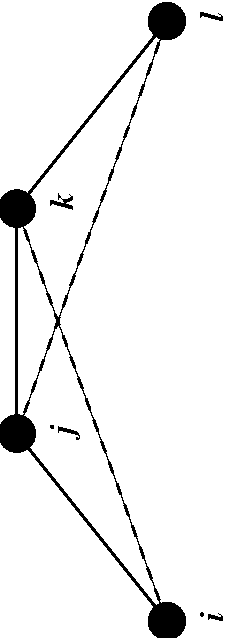
\includegraphics[angle=270,width=4cm]{plots/ring-imp}\hspace{1cm}
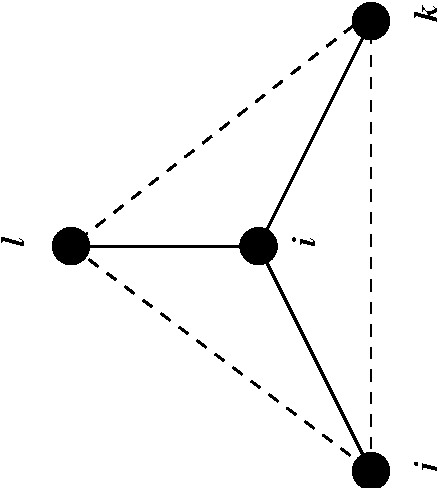
\includegraphics[angle=270,width=3cm]{plots/subst-im}\hspace{1cm}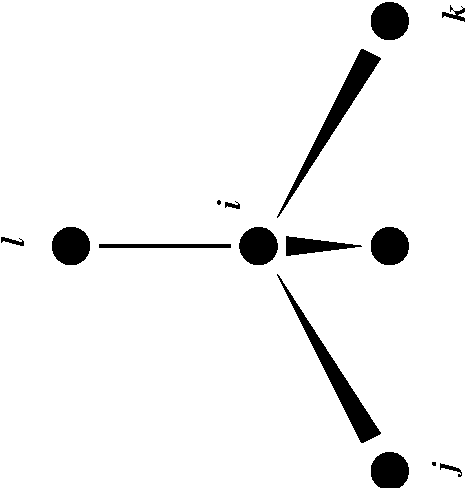
\includegraphics[angle=270,width=3cm]{plots/tetra-im}}
\caption[Improper dihedral angles.]{Principle of improper
dihedral angles. Out of plane bending for rings (left), substituents
of rings (middle), out of tetrahedral (right). The improper dihedral
angle $\xi$ is defined as the angle between planes (i,j,k) and (j,k,l)
in all cases.}
\label{fig:imp}
\end {figure}

\beq
V_{id}(\xi_{ijkl}) = \half k_{\xi}(\xi_{ijkl}-\xi_0)^2
\eeq
This is also a harmonic potential; it is plotted in
\figref{imps}. Note that, since it is harmonic, periodicity is
not taken into account, so it is best to define improper dihedrals
to have a $\xi_0$ as far away from $\pm 180^\circ$ as you can manage.

\begin{figure}
\centerline{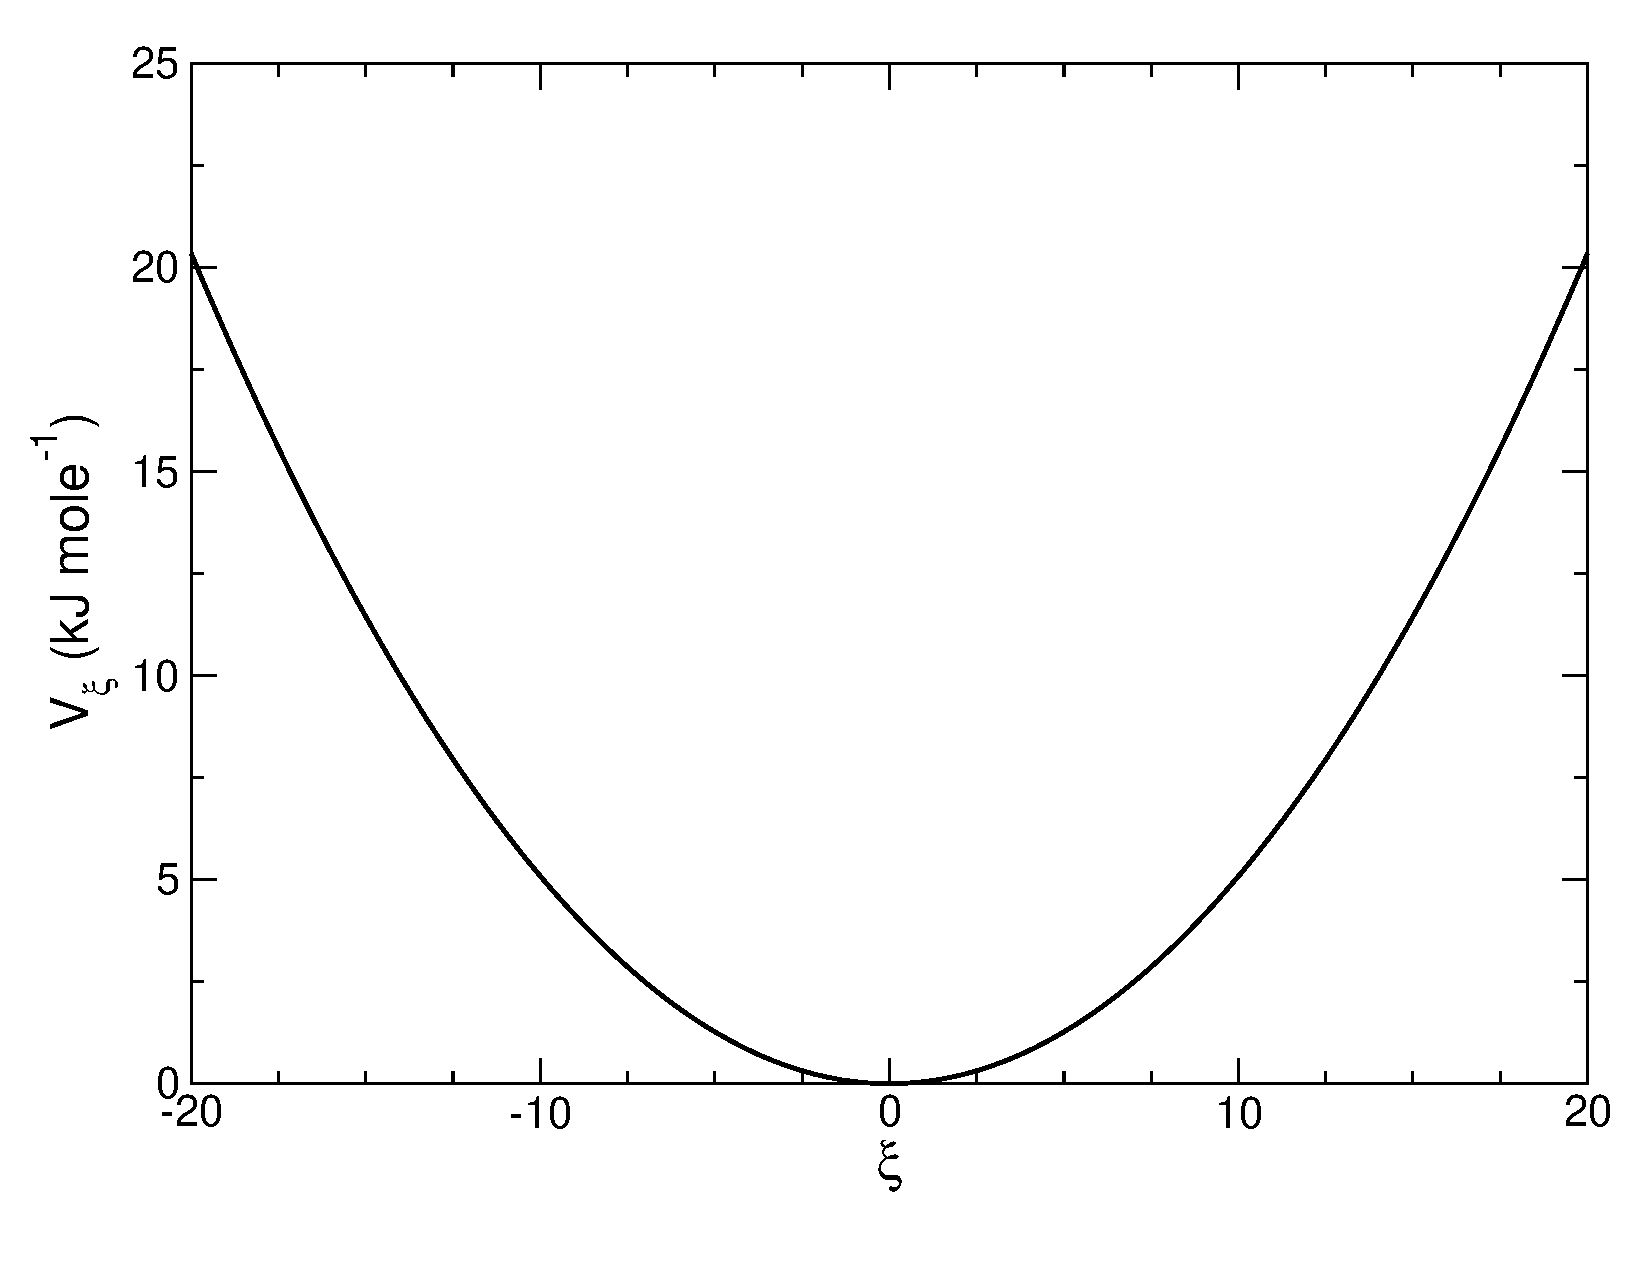
\includegraphics[angle=270,width=8cm]{plots/f_imps}}
\caption{Improper dihedral potential.}
\label{fig:imps}
\end{figure}

\subsection{Proper dihedrals}
For the normal \normindex{dihedral} interaction there is a choice of either the
{\gromos} periodic function or a function based on expansion in powers of
$\cos \phi$ (the so-called Ryckaert-Bellemans potential). This choice
has consequences for the inclusion of special interactions between the
first and the fourth atom of the dihedral quadruple. With the periodic
{\gromos} potential a special 1-4 LJ-interaction must be included; with
the Ryckaert-Bellemans potential the \normindex{1-4 interaction}s 
must be excluded from the non-bonded list.  

\subsubsection{Proper dihedrals: periodic type}
\swapindex{Proper}{dihedral} angles are defined according to the IUPAC/IUB
convention, where $\phi$ is the angle between the $ijk$ and the $jkl$
planes, with {\bf zero} corresponding to the {\em cis} configuration
($i$ and $l$ on the same side).

\begin{figure}
\centerline{\raisebox{-1cm}{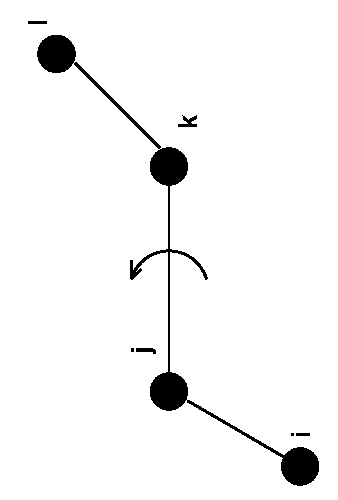
\includegraphics[angle=270,width=5cm]{plots/dih}}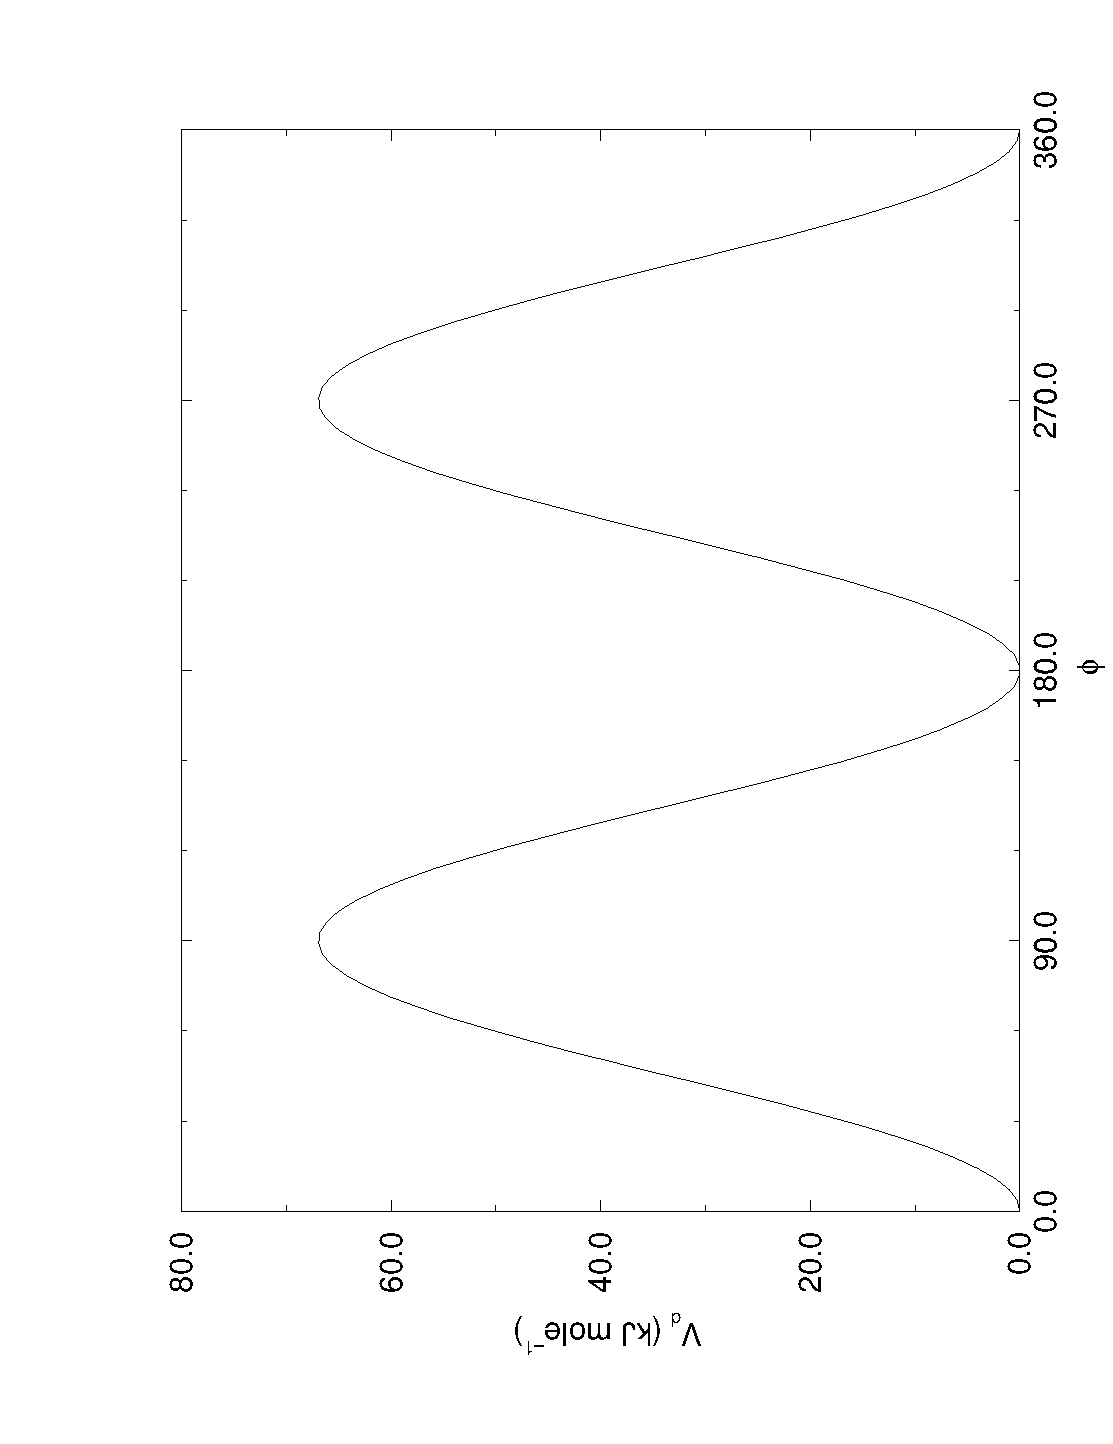
\includegraphics[angle=270,width=7cm]{plots/f_dih}}
\caption[Proper dihedral angle.]{Principle of proper dihedral angle
(left, in {\em trans} form) and the dihedral angle potential (right).} 
\label{fig:pdihf}
\end{figure}
\beq
V_d(\phi_{ijkl}) = k_{\phi}(1 + \cos(n \phi - \phi_s))
\eeq

\subsubsection{Proper dihedrals: Ryckaert-Bellemans function}
For alkanes, the following proper dihedral potential is often used
(see \figref{rbdih})
\beq
V_{rb}(\phi_{ijkl}) = \sum_{n=0}^5 C_n( \cos(\psi ))^n,
\eeq 
where $\psi = \phi - 180^\circ$.  \\
{\bf Note:} A conversion from one convention to another can be achieved by 
multiplying every coefficient \( \displaystyle C_n \) 
by \( \displaystyle (-1)^n \).

An example of constants for $C$ is given in \tabref{crb}.

\begin{table}
\centerline{
\begin{tabular}{|lr|lr|lr|}
\dline
$C_0$   & 9.28  & $C_2$   & -13.12  & $C_4$   & 26.24   \\
$C_1$   & 12.16 & $C_3$   & -3.06   & $C_5$   & -31.5   \\
\dline
\end{tabular}
}
\caption{Constants for Ryckaert-Bellemans potential (kJ mol$^{-1}$).}
\label{tab:crb}
\end{table}

\begin{figure}
\centerline{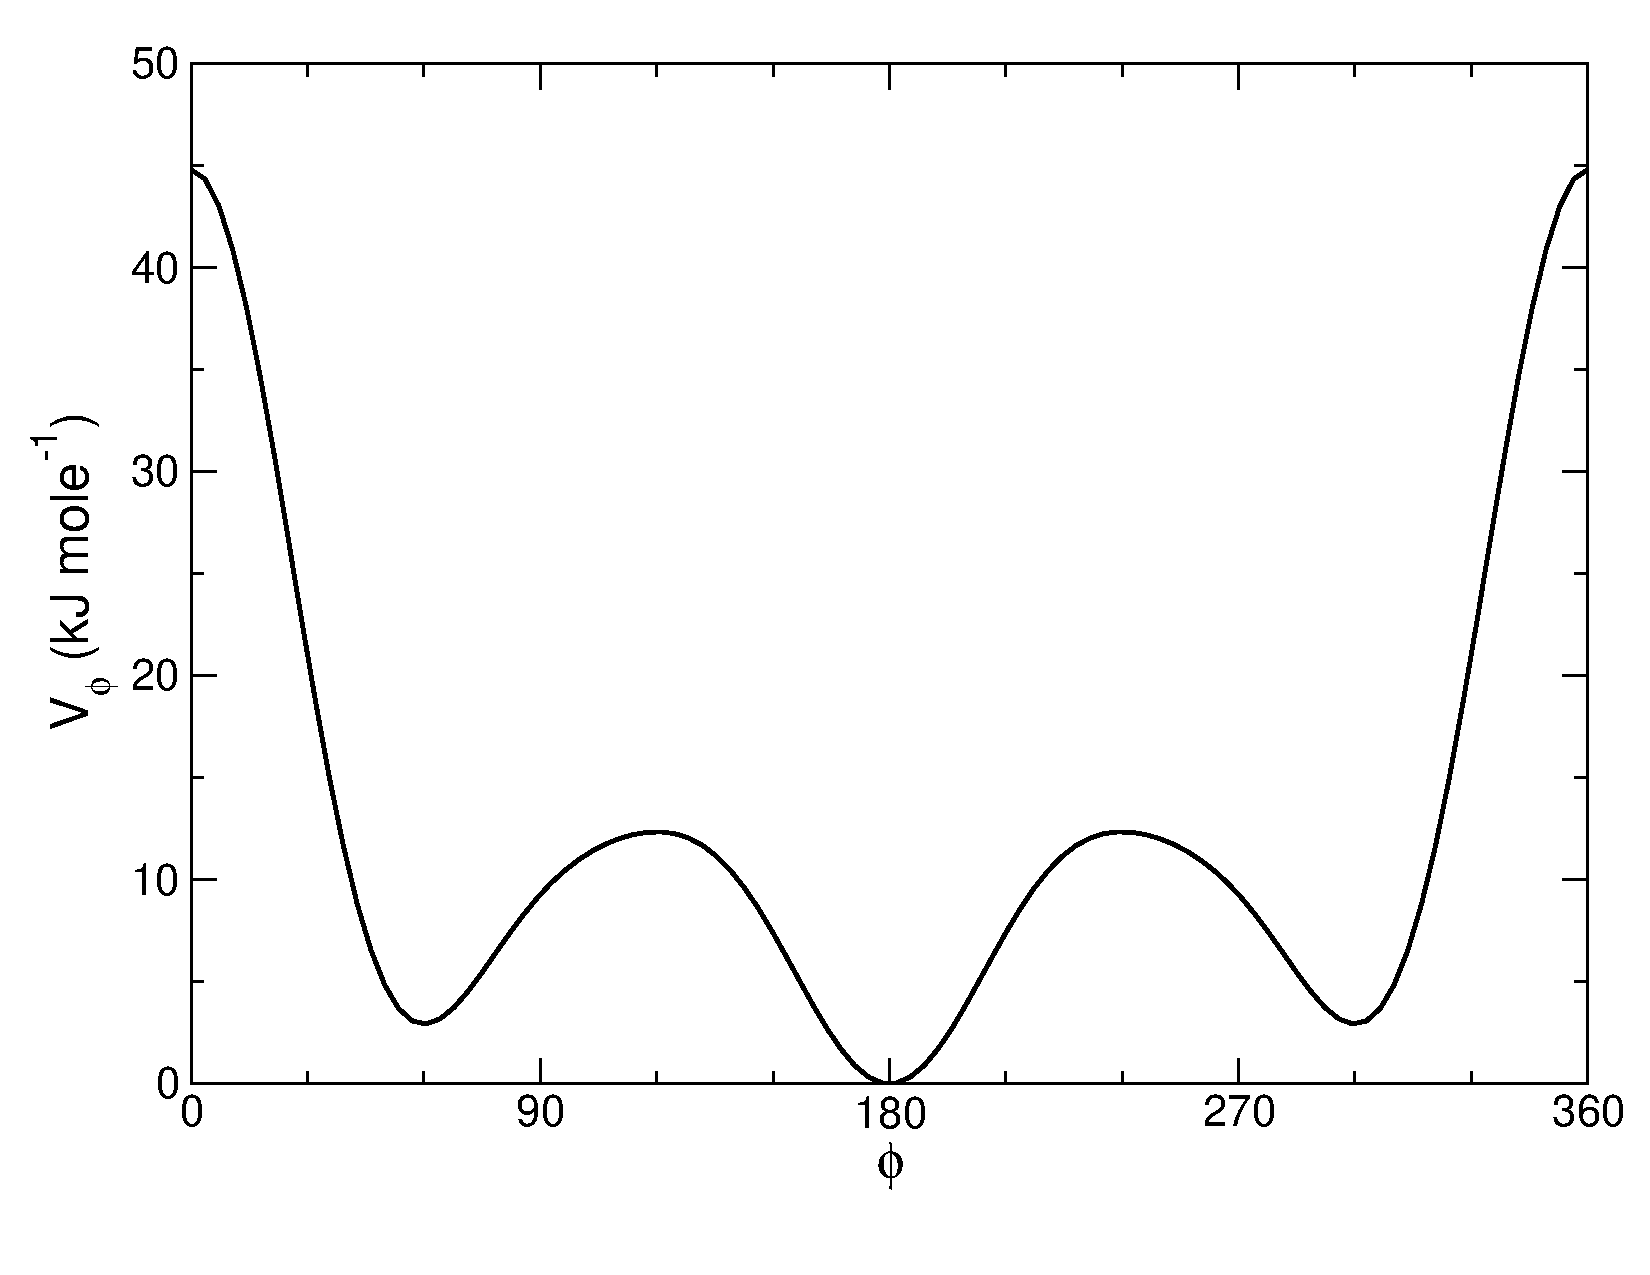
\includegraphics[angle=270,width=8cm]{plots/f_rbs}}
\caption{Ryckaert-Bellemans dihedral potential.}
\label{fig:rbdih}
\end{figure}

({\bf Note:} The use of this potential implies exclusion of LJ interactions
between the first and the last atom of the dihedral, and $\psi$ is defined
according to the 'polymer convention' ($\psi_{trans}=0$).)

The RB dihedral function can also be used to include the \normindex{OPLS} 
dihedral potential~\cite{Jorgensen88}. 
The OPLS potential function is given as the first 
four terms of a Fourier series:
\beq
V_{rb} (\phi_{ijkl}) ~=~ V_0 + \frac{1}{2} (V_1(1+\cos(\psi)) + V_2(
1-\cos(2\psi)) + V_3(1+\cos(3\psi))),
\eeq
with \( \displaystyle \psi=\phi \) (protein convention).
Because of the equalities \( \cos(2\phi) = 2(\cos(\phi))^2 - 1 \) 
and \( \cos(3\phi) = 4(\cos(\phi))^3 - 3\cos(\phi) \), 
one can translate the OPLS parameters to 
Ryckaert-Bellemans parameters as follows:
\beq
\displaystyle
\begin{array}{rcl}
\displaystyle C_0&=&V_0 + V_2 + \frac{1}{2} (V_1 + V_3)\\
\displaystyle C_1&=&\frac{1}{2} (3V_3 - V_1)\\
\displaystyle C_2&=&-V_2\\
\displaystyle C_3&=&-2V_3\\
\displaystyle C_4&=&0\\
\displaystyle C_5&=&0
\end{array}
\eeq
with OPLS parameters in protein convention and RB parameters in 
polymer convention.\\
\noindent{\bf Note:} Mind the conversion from {\em kcal mol$^{-1}$} for 
literature OPLS and RB parameters to {\em kJ mol$^{-1}$} in {\gromacs}.

\section{Restraints}
Special potentials are used for imposing restraints on the motion of
the system, either to avoid disastrous deviations, or to include
knowledge from experimental data. In either case they are not really
part of the force field and the reliability of the parameters is not
important. The potential forms, as implemented in {\gromacs}, are
mentioned just for the sake of completeness.

\subsection{\swapindex{Position}{restraint}s}
\label{sec:posre}
These are used to restrain particles to fixed reference positions
$\ve{R}_i$. They can be used during equilibration in order to avoid
too drastic rearrangements of critical parts ({\eg} to restrain motion
in a protein that is subjected to large solvent forces when the
solvent is not yet equilibrated). Another application is the
restraining of particles in a shell around a region that is simulated
in detail, while the shell is only approximated because it lacks
proper interaction from missing particles outside the
shell. Restraining will then maintain the integrity of the inner
part. For spherical shells it is a wise procedure to make the force
constant depend on the radius, increasing from zero at the inner
boundary to a large value at the outer boundary. This feature has
not, however, been implemented in {\gromacs}.
\newcommand{\unitv}[1]{\hat{\bf #1}}
\newcommand{\halfje}[1]{\frac{#1}{2}}

The following form is used: 
\beq
V_{pr}(\ve{r}_i) = \halfje{1}k_{pr}|\rvi-\ve{R}_i|^2
\eeq
The potential is plotted in \figref{posres}.

\begin{figure}
\centerline{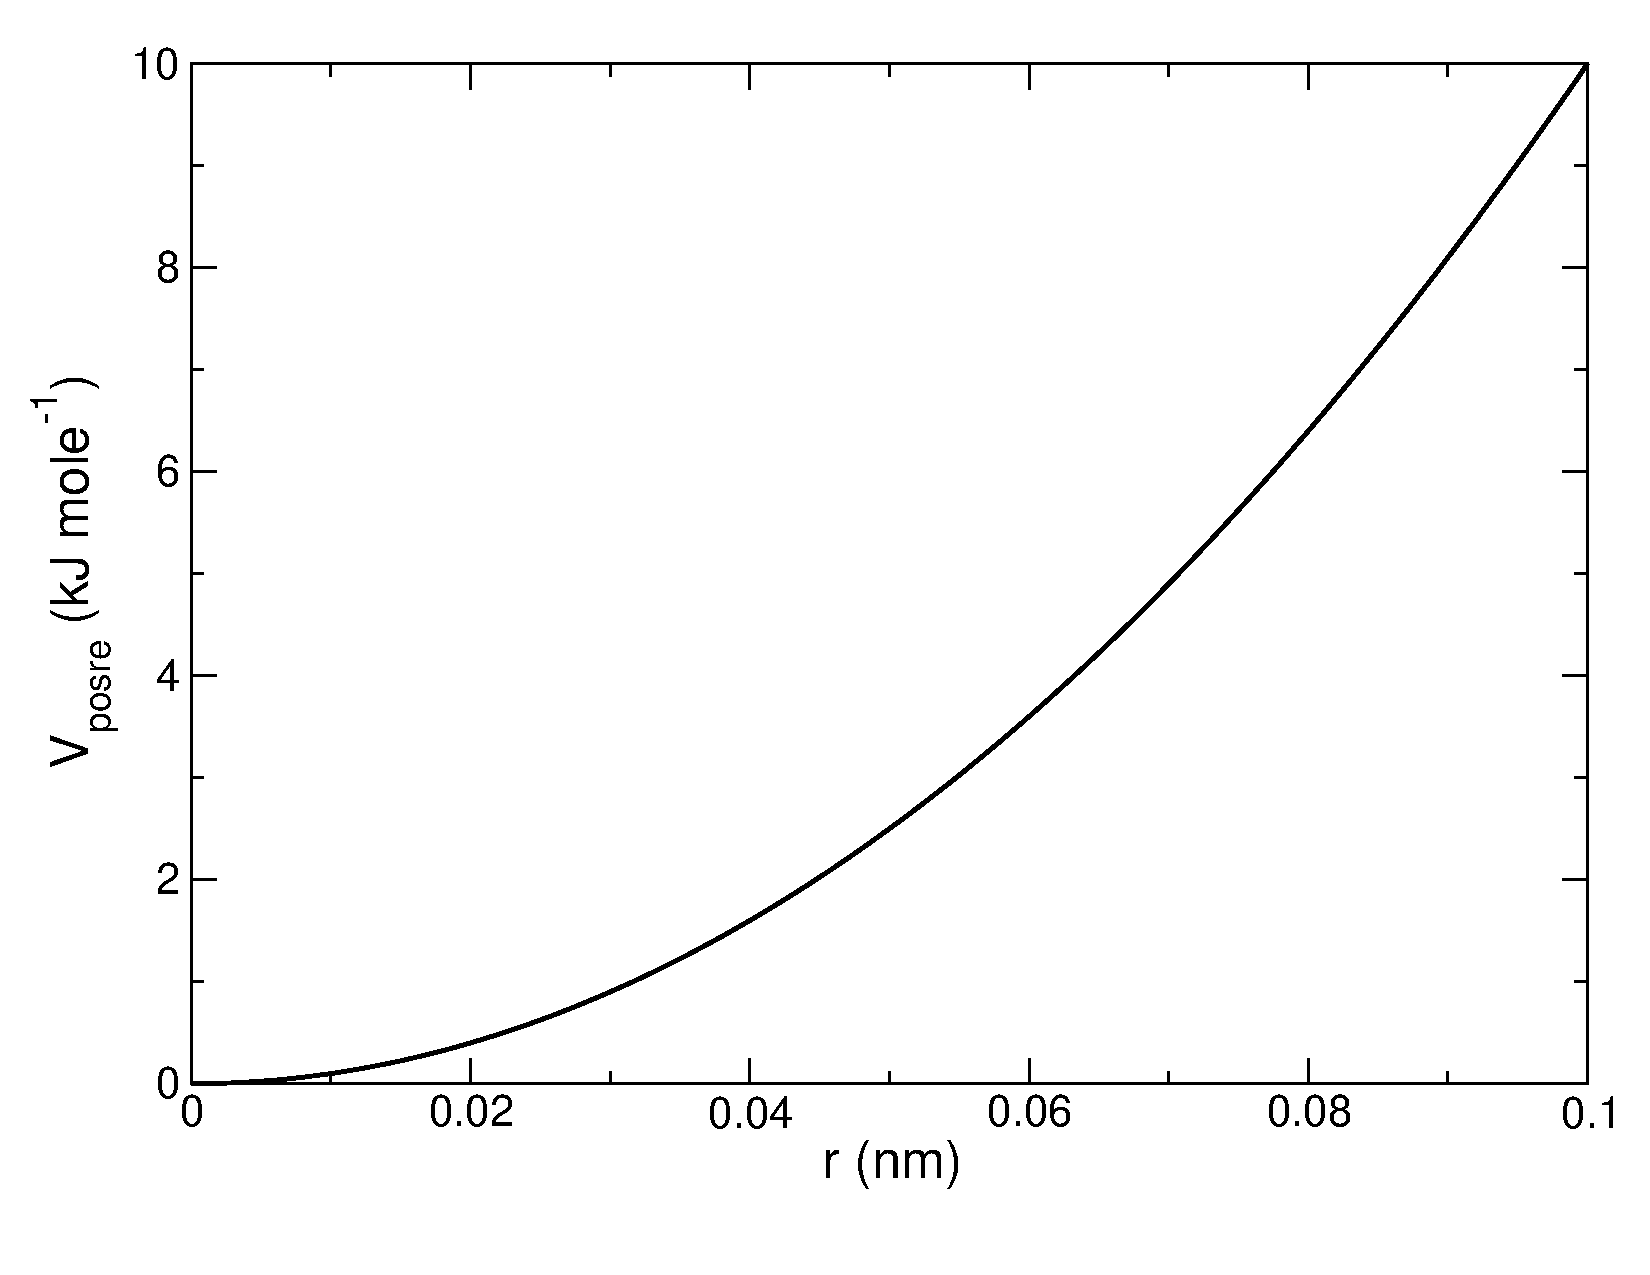
\includegraphics[angle=270,width=8cm]{plots/f_pr}}
\caption{Position restraint potential.}
\label{fig:posres}
\end{figure}

The potential form can be rewritten without loss of generality as:
\beq
V_{pr}(\ve{r}_i) = \halfje{1} \left[ k_{pr}^x (x_i-X_i)^2 ~\unitv{x} + k_{pr}^y (y_i-Y_i)^2 ~\unitv{y} + k_{pr}^z (z_i-Z_i)^2 ~\unitv{z}\right]
\eeq

Now the forces are:
\beq
\begin{array}{rcl}
F_i^x &=& -k_{pr}^x~(x_i - X_i) \\
F_i^y &=& -k_{pr}^y~(y_i - Y_i) \\
F_i^z &=& -k_{pr}^z~(z_i - Z_i)
\end{array}
\eeq
Using three different force constants the position 
restraints can be turned on or off
in each spatial dimension; this means that atoms can be harmonically
restrained to a plane or a line.
Position restraints are applied to a special fixed list of atoms. Such a
list is usually generated by the \normindex{pdb2gmx} program.

\subsection{\swapindex{Angle}{restraint}s}
\label{sec:angres}
These are used to restrain the angle between two pairs of particles
or between one pair of particles and the Z-axis.
The functional form is similar to that of a proper dihedral.
For two pairs of atoms: 
\beq
V_{ar}(\ve{r}_i,\ve{r}_j,\ve{r}_k,\ve{r}_l)
        = k_{ar}(1 - \cos(n (\theta - \theta_0))
        )
,~~~~\mbox{where}~~
\theta = \arccos\left(\frac{\ve{r}_j -\ve{r}_i}{\|\ve{r}_j -\ve{r}_i\|}
 \cdot \frac{\ve{r}_l -\ve{r}_k}{\|\ve{r}_l -\ve{r}_k\|} \right)
\eeq
For one pair of atoms and the Z-axis: 
\beq
V_{ar}(\ve{r}_i,\ve{r}_j) = k_{ar}(1 - \cos(n (\theta - \theta_0))
        )
,~~~~\mbox{where}~~
\theta = \arccos\left(\frac{\ve{r}_j -\ve{r}_i}{\|\ve{r}_j -\ve{r}_i\|}
 \cdot \left( \begin{array}{c} 0 \\ 0 \\ 1 \\ \end{array} \right) \right)
\eeq
A multiplicity ($n$) of 2 is useful when you do not want to distinguish
between parallel and anti-parallel vectors.


\subsection{\swapindex{Dihedral}{restraint}s}
\label{sec:dihres}
These are used to restrain the dihedral angle $\phi$ defined by four particles
as in an improper dihedral (sec.~\ref{sec:imp}) but with a slightly
modified potential. Using
\beq
\phi' = \left(\phi-\phi_0\right) ~{\rm MOD}~ 2\pi
\eeq
where $\phi_0$ is the reference angle, the potential is defined as:
\beq
V_{dihr}(\phi') ~=~ \left\{
\begin{array}{lcllll}
\half k_{dihr}(\phi'-\Delta\phi)^2      
                &\mbox{for}&     \phi' & >   & \Delta\phi       \\[1.5ex]
0               &\mbox{for}&     \phi' & \le & \Delta\phi       \\[1.5ex]
\end{array}\right.
\label{eqn:dihre}
\eeq
where $\Delta\phi$ is a user defined angle and $k_{dihr}$ is the force 
constant.

\subsection{\swapindex{Distance}{restraint}s}
\label{sec:disre}
Distance restraints 
add a penalty to the potential when the distance between specified
pairs of atoms exceeds a threshold value. They are normally used to
impose experimental restraints, as from experiments in nuclear
magnetic resonance (NMR), on the motion of the system. Thus MD can be
used for structure refinement using NMR data\index{nmr
refinement}\index{refinement,nmr}.
If one just wants to the restrain the distance between two particles
using a harmonic potential one should use {\tt [ bonds ]}
type 6 (see \ssecref{excl}).
The potential form for distance restraints is quadratic below a specified
lower bound and between two specified upper bounds and linear beyond the
largest bound (see \figref{dist}).
\beq
V_{dr}(r_{ij}) ~=~ \left\{
\begin{array}{lcllllll}
\half k_{dr}(r_{ij}-r_0)^2      
                &\mbox{for}&     &     & r_{ij} & < & r_0       \\[1.5ex]
0               &\mbox{for}& r_0 & \le & r_{ij} & < & r_1       \\[1.5ex]
\half k_{dr}(r_{ij}-r_1)^2      
                &\mbox{for}& r_1 & \le & r_{ij} & < & r_2       \\[1.5ex]
\half k_{dr}(r_2-r_1)(2r_{ij}-r_2-r_1)  
                &\mbox{for}& r_2 & \le & r_{ij} &   &
\end{array}\right.
\label{eqn:disre}
\eeq

\begin{figure}
\centerline{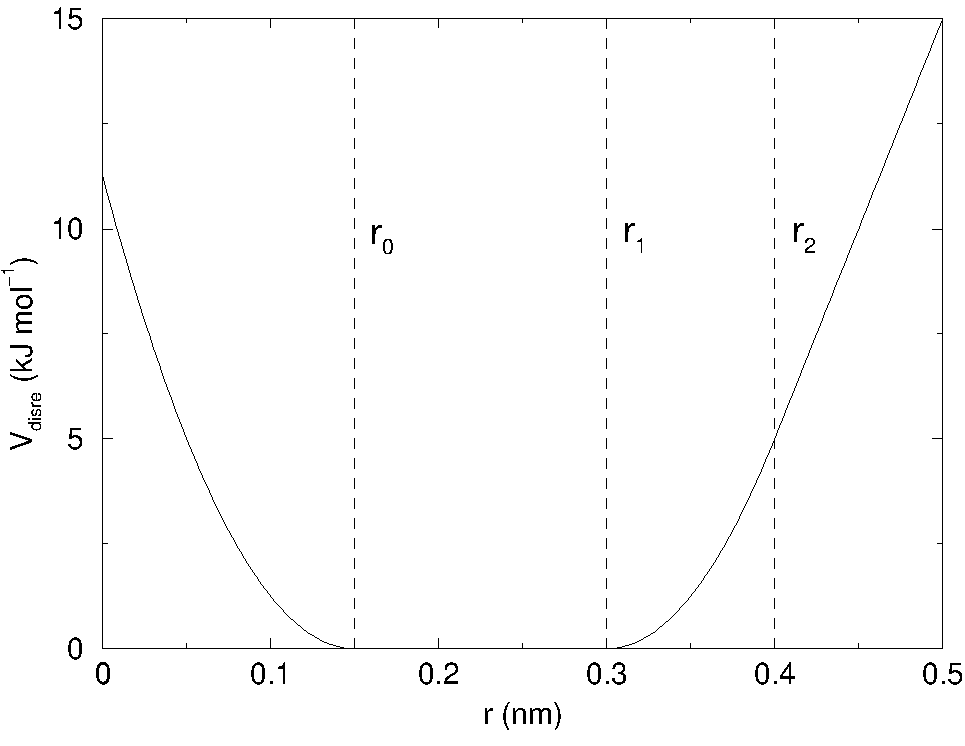
\includegraphics[width=8cm]{plots/f_dr}}
\caption{Distance Restraint potential.}
\label{fig:dist}
\end{figure}

The forces are
\beq
\ve{F}_i~=~ \left\{
\begin{array}{lcllllll}
-k_{dr}(r_{ij}-r_0)\frac{\rvij}{r_{ij}} 
                &\mbox{for}&     &     & r_{ij} & < & r_0       \\[1.5ex]
0               &\mbox{for}& r_0 & \le & r_{ij} & < & r_1       \\[1.5ex]
-k_{dr}(r_{ij}-r_1)\frac{\rvij}{r_{ij}} 
                &\mbox{for}& r_1 & \le & r_{ij} & < & r_2       \\[1.5ex]
-k_{dr}(r_2-r_1)\frac{\rvij}{r_{ij}}    
                &\mbox{for}& r_2 & \le & r_{ij} &   &
\end{array} \right.
\eeq

\subsubsection{Time averaging}
Distance restraints based on instantaneous distances can potentially reduce
the fluctuations in a molecule significantly. This problem can be overcome by restraining
to a {\em time averaged} distance~\cite{Torda89}.
The forces with time averaging are:
\beq
\ve{F}_i~=~ \left\{
\begin{array}{lcllllll}
-k^a_{dr}(\bar{r}_{ij}-r_0)\frac{\rvij}{r_{ij}}   
                &\mbox{for}&     &     & \bar{r}_{ij} & < & r_0 \\[1.5ex]
0               &\mbox{for}& r_0 & \le & \bar{r}_{ij} & < & r_1 \\[1.5ex]
-k^a_{dr}(\bar{r}_{ij}-r_1)\frac{\rvij}{r_{ij}}   
                &\mbox{for}& r_1 & \le & \bar{r}_{ij} & < & r_2 \\[1.5ex]
-k^a_{dr}(r_2-r_1)\frac{\rvij}{r_{ij}}    
                &\mbox{for}& r_2 & \le & \bar{r}_{ij} &   &
\end{array} \right.
\eeq
where $\bar{r}_{ij}$ is given by an exponential running average with decay time $\tau$:
\beq
\bar{r}_{ij} ~=~ < r_{ij}^{-3} >^{-1/3}
\label{eqn:rav}
\eeq
and the force constant $k^a_{dr}$ is switched on slowly to compensate for
the lack of history at the beginning of the simulation:
\beq
k^a_{dr} = k_{dr} \left(1-\exp\left(-\frac{t}{\tau}\right)\right)
\eeq
Because of the time averaging we can no longer speak of a distance restraint
potential.

This way an atom can satisfy two incompatible distance restraints 
{\em on average} by moving between two positions. 
An example would be an amino-acid side-chain which is rotating around
its $\chi$ dihedral angle, thereby coming close to various other groups.
Such a mobile side chain can give rise to multiple NOEs that can not be
fulfilled by a single structure.

The computation of the time
averaged distance in the {\tt mdrun} program is done in the following fashion:
\beq
\begin{array}{rcl}
\overline{r^{-3}}_{ij}(0)       &=& r_{ij}(0)^{-3}      \\
\overline{r^{-3}}_{ij}(t)       &=& \overline{r^{-3}}_{ij}(t-\Delta t)~\exp{\left(-\frac{\Delta t}{\tau}\right)} + r_{ij}(t)^{-3}\left[1-\exp{\left(-\frac{\Delta t}{\tau}\right)}\right]
\label{eqn:ravdisre}
\end{array}
\eeq

When a pair is within the bounds it can still feel a force,
because the time averaged distance can still be beyond a bound.
To prevent the protons from being pulled too close together a mixed
approach can be used. In this approach the penalty is zero when the
instantaneous distance is within the bounds, otherwise the violation is
the square root of the product of the instantaneous violation and the 
time averaged violation:
\beq
\ve{F}_i~=~ \left\{
\begin{array}{lclll}
k^a_{dr}\sqrt{(r_{ij}-r_0)(\bar{r}_{ij}-r_0)}\frac{\rvij}{r_{ij}}   
    & \mbox{for} & r_{ij} < r_0 & \mbox{and} & \bar{r}_{ij} < r_0 \\[1.5ex]
-k^a _{dr} \,
  \mbox{min}\left(\sqrt{(r_{ij}-r_1)(\bar{r}_{ij}-r_1)},r_2-r_1\right)
  \frac{\rvij}{r_{ij}}   
    & \mbox{for} & r_{ij} > r_1 & \mbox{and} & \bar{r}_{ij} > r_1 \\[1.5ex]
0               &\mbox{else}
\end{array} \right.
\eeq

\subsubsection{Averaging over multiple pairs} 

Sometimes it is unclear from experimental data which atom pair
gives rise to a single NOE, in other occasions it can be obvious that
more than one pair contributes due to the symmetry of the system, {\eg} a
methyl group with three protons. For such a group it is not possible 
to distinguish between the protons, therefore they should all be taken into
account when calculating the distance between this methyl group and another
proton (or group of protons).
Due to the physical nature of magnetic resonance, the intensity of the
NOE signal is inversely proportional to the sixth power of the interatomic 
distance.
Thus, when combining atom pairs, 
a fixed list of $N$ restraints may be taken together, 
where the apparent ``distance'' is given by:
\beq
r_N(t) = \left [\sum_{n=1}^{N} \bar{r}_{n}(t)^{-6} \right]^{-1/6}
\label{eqn:rsix}
\eeq
where we use $r_{ij}$ or \eqnref{rav} for the $\bar{r}_{n}$.
The $r_N$ of the instantaneous and time-averaged distances
can be combined to do a mixed restraining as indicated above.
As more pairs of protons contribute to the same NOE signal, the intensity
will increase, and the summed ``distance'' will be shorter than any of
its components due to the reciprocal summation. 

There are two options for distributing the forces over the atom pairs.
In the conservative option the force is defined as the derivative of the
restraint potential with respect to the coordinates. This results in
a conservative potential when time averaging is not used.
The force distribution over the pairs is proportional to $r^{-6}$.
This means that a close pair feels a much larger force than a distant pair,
which might lead to a 'too rigid' molecule.
The other option is an equal force distribution. In this case each pair
feels $1/N$ of the derivative of the restraint potential with respect to 
$r_N$. The advantage of this method is that more conformations might be
sampled, but the non-conservative nature of the forces can lead to
local heating of the protons.

It is also possible to use {\em ensemble averaging} using multiple
(protein)  molecules. In this case the bounds should be lowered as in:
\beq
\begin{array}{rcl}
r_1     &~=~&   r_1 * M^{-1/6}  \\
r_2     &~=~&   r_2 * M^{-1/6}
\end{array}
\eeq
where $M$ is the number of molecules. The {\gromacs} preprocessor {\tt grompp}
can do this automatically when the appropriate option is given.
The resulting ``distance'' is 
then used to calculate the scalar force according to:
\beq
\begin{array}{rcl}
\ve{F}_i~=~&~0 \hspace{4cm}  & r_{N} < r_1         \\
  = ~&-~ k_{dr}(r_{N}-r_1)\frac{\rvij}{r_{ij}} & r_1 \le r_{N} < r_2 \\
  = ~&-~ k_{dr}(r_2-r_1)\frac{\rvij}{r_{ij}}    & r_{N} \ge r_2 
\end{array}
\eeq
where $i$ and $j$ denote the atoms of all the 
pairs that contribute to the NOE signal.

\subsubsection{Using distance restraints}

A list of distance restrains based on NOE data can be added to a molecule
definition in your topology file, like in the following example:
\begin{verbatim}
[ distance_restraints ]
; ai   aj    type  index  type'   low    up1    up2    fac
10     16     1      0      1     0.0    0.3    0.4    1.0 
10     28     1      1      1     0.0    0.3    0.4    1.0 
10     46     1      1      1     0.0    0.3    0.4    1.0 
16     22     1      2      1     0.0    0.3    0.4    2.5 
16     34     1      3      1     0.0    0.5    0.6    1.0 
\end{verbatim}
In this example a number of features can be found.  In columns {\tt
ai} and {\tt aj} you find the atom numbers of the particles to be
restrained. The {\tt type} column should always be 1.  As explained in
~\secref{disre}, multiple distances can contribute to a single NOE
signal. In the topology this can be set using the {\tt index}
column. In our example, the restraints 10-28 and 10-46 both have index
1, therefore they are treated simultaneously.  An extra requirement
for treating restraints together, is that the restraints should be on
successive lines, without any other intervening restraint.  The {\tt
type'} column will usually be 1, but can be set to 2 to obtain a
distance restraint which will never be time and ensemble averaged;
this can be useful for restraining hydrogen bonds.  The columns {\tt
low}, {\tt up1} and {\tt up2} hold the values of $r_0$, $r_1$ and
$r_2$ from ~\eqnref{disre}.  In some cases it can be useful to have
different force constants for some restraints; this is controlled by
the column {\tt fac}.  The force constant in the parameter file is
multiplied by the value in the column {\tt fac} for each restraint.

Some parameters for NMR refinement can be specified in the
{\tt grompp.mdp} file:
\begin{description}
\item[{\tt disre}: type of distance restraining.]
        The {\tt disre} variable sets the type of distance restraint.
        {\tt no/simple} turns the distance restraints off/on.
        When multiple proteins or peptides are present in one 
        simulation box, ensemble averaging 
        can be turned on by setting {\tt disre = ensemble}.
	Normally one would perform ensemble averaging over multiple
	subsystems, each in a separate box, using {\tt mdrun -multi};
	supply {\tt topol0.tpr}, {\tt topol1.tpr}, ... with different
	coordiates and/or velocities.
\item[{\tt disre\_weighting}: force-weighting in restraints with
         multiple pairs.]
        By default, the force due to the distance restraint is distributed equally
        over all the pairs involved in the restraint. This can also be
        explicitly selected with
        {\tt disre\_weighting = equal}. 
        If you instead set this option to {\tt disre\_weighting = conservative}
        you get conservative forces when {\tt disre\_tau = 0}.
\item[{\tt disre\_mixed}: how to calculate the violations.]
        {\tt disre\_mixed = no} gives normal time-averaged violations.
        When {\tt disre\_mixed = yes} the square root of the
        product of the time-averaged and the instantaneous
        violations is used.
\item[{\tt disre\_fc}: force constant $k_{dr}$ for distance restraints.] 
        $k_{dr}$  (\eqnref{disre}) can be set
        as variable {\tt disre\_fc = 1000} for a force constant of
        1000 {kJ mol$^{-1}$ nm$^{-2}$}. This value is multiplied by
        the value in the {\tt fac} column in the distance restraint
        entries in the topology file.
\item[{\tt disre\_tau}: time constant for restraints.] 
        $\tau$ (\eqnref{ravdisre}) can be set
        as variable {\tt disre\_tau = 10} for a time constant of
        10 ps. Time averaging can be turned off by setting {\tt disre\_tau}
        to 0.
\item[{\tt nstdisreout}: pair distance output frequency.]
        Determines how often the time-averaged and 
        instantaneous distances of all atom pairs involved in
        distance restraints are written to the energy file.
\end{description}

\newcommand{\SSS}{{\mathbf S}}
\newcommand{\DD}{{\mathbf D}}
\newcommand{\RR}{{\mathbf R}}

\subsection{\swapindex{Orientation}{restraint}s}
\label{sec:orire}
This section describes how orientations between vectors,
as measured in certain NMR experiments, can be calculated
and restrained in MD simulations.
The presented refinement methodology and a comparision of results
with and without time and ensemble averaging have been
published~\cite{Hess2003}.
\subsubsection{Theory}
In an NMR experiment orientations of vectors can be measured when a 
molecule does not tumble completely isotropically in the solvent.
Two examples of such orientation measurements are
residual \normindex{dipolar couplings}
(between two nuclei) or chemical shift anisotropies.
An observable for a vector $\ve{r}_i$ can be written as follows:
\beq
\delta_i = \frac{2}{3} \mbox{tr}(\SSS\DD_i)
\eeq
where $\SSS$ is the dimensionless order tensor of the molecule.
The tensor $\DD_i$ is given by:
\beq
\label{orient_def}
\DD_i = \frac{c_i}{\|\ve{r}_i\|^\alpha} \left(
%\begin{array}{lll}
%3 r_x r_x - \ve{r}\cdot\ve{r} & 3 r_x r_y & 3 r_x r_z \\
%3 r_x r_y                     & 3 r_y r_y - \ve{r}\cdot\ve{r} & 3yz \\
%3 r_x r_z                     & 3 r_y r_z & 3 r_z r_z - \ve{r}\cdot\ve{r}
%\end{array} \right)
\begin{array}{lll}
3 x x - 1 & 3 x y     & 3 x z     \\
3 x y     & 3 y y - 1 & 3 y z     \\
3 x z     & 3 y z     & 3 z z - 1 \\
\end{array} \right)
\eeq
\beq
\mbox{with:} \quad 
x=\frac{r_{i,x}}{\|\ve{r}_i\|}, \quad
y=\frac{r_{i,y}}{\|\ve{r}_i\|}, \quad 
z=\frac{r_{i,z}}{\|\ve{r}_i\|}
\eeq
For a dipolar coupling $\ve{r}_i$ is the vector connecting the two
nuclei, $\alpha=3$ and the constant $c_i$ is given by:
\beq
c_i = \frac{\mu_0}{4\pi} \gamma_1^i \gamma_2^i \frac{\hbar}{4\pi}
\eeq
where $\gamma_1^i$ and $\gamma_2^i$ are the gyromagnetic ratios of the
two nuclei.

The order tensor is symmetric and has trace zero. Using a rotation matrix
${\mathbf T}$ it can be transformed into the following form:
\beq
{\mathbf T}^T \SSS {\mathbf T} = s \left( \begin{array}{ccc}
-\frac{1}{2}(1-\eta) & 0                    & 0 \\
0                    & -\frac{1}{2}(1+\eta) & 0 \\
0                    & 0                    & 1
\end{array} \right)
\eeq
where $-1 \leq s \leq 1$ and $0 \leq \eta \leq 1$.
$s$ is called the order parameter and $\eta$ the asymmetry of the
order tensor $\SSS$. When the molecule tumbles isotropically in the
solvent $s$ is zero and no orientational effects can be observed
as all $\delta_i$ are zero.

%\newpage

\subsubsection{Calculating orientations in a simulation}
For reasons which are explained below, the $\DD$ matrices are calculated
which respect to a reference orientation of the molecule. The orientation
is defined by a rotation matrix $\RR$ which is needed to least-squares fit
the current coordinates of a selected set of atoms onto
a reference conformation. The reference conformation is the starting
conformation of the simulation. In case of ensemble averaging, which will
be treated later, the structure is taken from the first subsystem.
The calculated $\DD_i^c$ matrix is given by:
\begin{equation}
\label{D_rot}
\DD_i^c(t) = \RR(t) \DD_i(t) \RR^T(t)
\end{equation}
The calculated orientation for vector $i$ is given by:
\beq
\delta^c_i(t) = \frac{2}{3} \mbox{tr}(\SSS(t)\DD_i^c(t))
\eeq
The order tensor $\SSS(t)$ is usually unknown.
A reasonable choice for the order tensor is the tensor
which minimizes the (weighted) mean square difference between the calculated
and the observed orientations:
\begin{equation}
\label{S_msd}
MSD(t) = \left(\sum_{i=1}^N w_i\right)^{-1} \sum_{i=1}^N w_i (\delta_i^c (t) -\delta_i^{exp})^2
\end{equation}
To properly combine different types of measurements the unit of $w_i$ should
be such that all terms are dimensionless. This means the unit of $w_i$
is the unit of $\delta_i$ to the power $-2$.
Note that scaling all $w_i$ with a constant factor does not influence
the order tensor.

\subsubsection{Time averaging}
Since the tensors $\DD_i$ fluctuate rapidly in time, much faster than can
be observed in experiment, they should be time averaged in the simulation.
However, in a simulation the time as well as the number of copies of
a molecule is limited. Usually one can not obtain a converged average
of the $\DD_i$ tensors over all orientations of the molecule.
If one assumes that the average orientations of the $\ve{r}_i$ vectors
within the molecule converge much faster than the tumbling time of
the molecule, the tensor can be averaged in an axis system which
rotates with the molecule, as expressed by equation~(\ref{D_rot}).
The time averaged tensors are calculated
using an exponentially decaying memory function:
\beq
\DD^a_i(t) = \frac{\displaystyle
\int_{u=t_0}^t \DD^c_i(u) \exp\left(-\frac{t-u}{\tau}\right)\mbox{d} u
}{\displaystyle
\int_{u=t_0}^t \exp\left(-\frac{t-u}{\tau}\right)\mbox{d} u
}
\eeq
Assuming that the order tensor $\SSS$ fluctuates slower than the
$\DD_i$, the time averaged orientation can be calculated as:
\beq
\delta_i^a(t) = \frac{2}{3} \mbox{tr}(\SSS(t) \DD_i^a(t))
\eeq
where the order tensor $\SSS(t)$ is calculated using expression~(\ref{S_msd})
with $\delta_i^c(t)$ replaced by $\delta_i^a(t)$.

\subsubsection{Restraining}
The simulated structure can be restrained by applying a force proportional
to the difference between the calculated and the experimental orientations.
When no time averaging is applied a proper potential can be defined as:
\beq
V = \frac{1}{2} k \sum_{i=1}^N w_i (\delta_i^c (t) -\delta_i^{exp})^2
\eeq
where the unit of $k$ is the unit of energy.
Thus the effective force constant for restraint $i$ is $k w_i$.
The forces are given by minus the gradient of $V$.
The force $\ve{F}\!_i$ working on vector $\ve{r}_i$ is:
\begin{eqnarray*}
\ve{F}\!_i(t) 
& = & - \frac{\mbox{d} V}{\mbox{d}\ve{r}_i} \\
& = & -k w_i (\delta_i^c (t) -\delta_i^{exp}) \frac{\mbox{d} \delta_i (t)}{\mbox{d}\ve{r}_i} \\
& = & -k w_i (\delta_i^c (t) -\delta_i^{exp})
\frac{2 c_i}{\|\ve{r}\|^{2+\alpha}} \left(2 \RR^T \SSS \RR \ve{r}_i - \frac{2+\alpha}{\|\ve{r}\|^2} \mbox{tr}(\RR^T \SSS \RR \ve{r}_i \ve{r}_i^T) \ve{r}_i \right)
\end{eqnarray*}

\subsubsection{Ensemble averaging}
Ensemble averaging can be applied by simulating a system of $M$ subsystems
which each contain an identical set of orientation restraints. The systems only
interact via the orientation restraint potential which is defined as:
\beq
V = M \frac{1}{2} k \sum_{i=1}^N w_i 
\langle \delta_i^c (t) -\delta_i^{exp} \rangle^2
\eeq
The force on vector $\ve{r}_{i,m}$ in subsystem $m$ is given by:
\beq
\ve{F}\!_{i,m}(t) = - \frac{\mbox{d} V}{\mbox{d}\ve{r}_{i,m}} =
-k w_i \langle \delta_i^c (t) -\delta_i^{exp} \rangle \frac{\mbox{d} \delta_{i,m}^c (t)}{\mbox{d}\ve{r}_{i,m}} \\
\eeq 

\subsubsection{Time averaging}
When using time averaging it is not possible to define a potential.
We can still define a quantity which gives a rough idea of the energy
stored in the restraints:
\beq
V = M \frac{1}{2} k^a \sum_{i=1}^N w_i 
\langle \delta_i^a (t) -\delta_i^{exp} \rangle^2
\eeq
The force constant $k_a$ is switched on slowly to compensate for the
lack of history at times close to $t_0$. It is exactly proportional
to the amount of average which has been accumulated:
\beq
k^a =
 k \, \frac{1}{\tau}\int_{u=t_0}^t \exp\left(-\frac{t-u}{\tau}\right)\mbox{d} u
\eeq
What really matters is the definition of the force. It is chosen to
be proportional to the square root of the product of the time averaged
and the instantaneous deviation.
Using only the time averaged deviation induces large oscillations.
The force is given by:
\beq
\ve{F}\!_{i,m}(t) =
%\left\{ \begin{array}{ll}
%0 & \mbox{for} \quad \langle \delta_i^a (t) -\delta_i^{exp} \rangle \langle \delta_i (t) -\delta_i^{exp} \rangle \leq 0 \\
%... & \mbox{for} \quad \langle \delta_i^a (t) -\delta_i^{exp} \rangle \langle \delta_i (t) -\delta_i^{exp} \rangle > 0 
%\end{array}
%\right.
\left\{ \begin{array}{ll}
0 & \quad \mbox{for} \quad a\, b \leq 0 \\
\displaystyle
k^a w_i \frac{a}{|a|} \sqrt{a\, b} \, \frac{\mbox{d} \delta_{i,m}^c (t)}{\mbox{d}\ve{r}_{i,m}}
& \quad \mbox{for} \quad a\, b > 0 
\end{array}
\right.
\eeq
\begin{eqnarray*}
a &=& \langle \delta_i^a (t) -\delta_i^{exp} \rangle \\
b &=& \langle \delta_i^c (t) -\delta_i^{exp} \rangle
\end{eqnarray*}

\subsubsection{Using orientation restraints}
Orientation restraints can be added to a molecule definition in
the topology in the section {\tt [ orientation\_restraints ]}.
Here we give an example section containing five N-H residual dipolar
coupling restraints:
\begin{verbatim}
[ orientation_restraints ]
; ai   aj type exp. label alpha   const.    obs.  weight 
;                                Hz nm^3      Hz  1/Hz^2
  31   32    1    1     3     3    6.083   -6.73     1.0
  43   44    1    1     4     3    6.083   -7.87     1.0
  55   56    1    1     5     3    6.083   -7.13     1.0
  65   66    1    1     6     3    6.083   -2.57     1.0
  73   74    1    1     7     3    6.083   -2.10     1.0
\end{verbatim}
The unit of the observable is Hz, but one can choose any other unit.
In columns {\tt
ai} and {\tt aj} you find the atom numbers of the particles to be
restrained. The {\tt type} column should always be 1.
The {\tt exp.} column denotes the experiment number, this starts
numbering at 1. For each experiment a separate order tensor $\SSS$
is optimized. The label should be a unique number larger than zero
for each restraint. The {\tt alpha} column contains the power $\alpha$ 
which is used in equation~(\ref{orient_def}) to calculate the orientation.
The {\tt const.} column contains the constant $c_i$ used in the same
equation. The constant should have the unit of the observable times
nm$^\alpha$. The column {\tt obs.} contains the observable, in any
unit you like. The last column contains the weights $w_i$, the unit
should be the inverse of the square of the unit of the observable.

Some parameters for orientation restraints can be specified in the
{\tt grompp.mdp} file, for a study of the effect of different
force constants and averaging times and ensemble averaging see~\cite{Hess2003}.
\begin{description}
\item[{\tt orire}: use orientation restraining.]
        {\tt no/yes} turns the distance restraints off/on.
	Ensemble averaging can be performed using {\tt mdrun -multi},
	which simulates multiple subsystems in separate boxes;
	supply {\tt topol0.tpr}, {\tt topol1.tpr}, ... with different
	coordiates and/or velocities.
\item[{\tt orire\_fc}: force constant $k$ for orientation restraints.] 
	The unit of $k$ is kJ mol$^{-1}$.
	Note that the force constant for a restraint is this force constant
	times the weight of the restraint.
	When set to zero one obtain the calculated orientation without
	affecting the simulation.
\item[{\tt orire\_tau}: time constant $\tau$ for restraints.] 
        Set {\tt orire\_tau = 10} for a time constant of
        10 ps. Time averaging can be turned off by setting {\tt orire\_tau}
        to 0.
\item[{\tt orire\_fitgrp}: the fit group for the restraints.]
	This group of atoms is used to determine the rotation $\RR$
	of the system with respect to the reference orientation.
	The reference orientation is the starting conformation of
	the first subsystem. For a protein {\tt backbone} should be
        a reasonable choice.	
\item[{\tt nstorireout}: orientation output frequency.]
        Determines how often the orientations for all restraints
        and the order tensor(s) $\SSS$ are written to the energy file.
	When using time and/or ensemble averaging, the time and ensemble
	averaged orientations as well as the instantaneous non-ensemble
	averaged orientations are written to the energy file.
	These can be analyzed using {\tt g\_energy}.
\end{description}

\section{Polarization}
Polarization can be treated by {\gromacs} by attaching
\normindex{shell} (\normindex{drude}) particles to atoms and/or
virtual sites. The energy of the shell particle is then minimized at
each time step in order to remain on the Born-Oppenheimer surface.

\subsection{Simple polarization}
This is merely a harmonic potential with equilibrium distance 0.

\subsection{Water polarization}
A special potential for water that allows anisotropic polarization of
a single shell particle~\cite{Maaren2001a}.

\subsection{Thole polarization}
Based on early work by \normindex{Thole}~\cite{Thole81} Roux and
coworkers have implemented potentials for molecules like
ethanol~\cite{Lamoureux2003a,Lamoureux2003b,Noskov2005a}. Within such
molecules there are intramolecular interaction between shell
particles, however these must be screened because full Coulomb would
be too strong. The potential between two shell particles $i$ and $j$ is:
\newcommand{\rbij}{\bar{r_{ij}}}
\beq
V_{thole} ~=~ \frac{q_i q_j}{r_{ij}}\left[1-\left(1-\frac{\rbij}{2}\right){\rm exp}^{-\rbij}\right]
\eeq
where
\beq
\rbij ~=~ a\frac{r_{ij}}{(\alpha_i \alpha_j)^{1/6}}
\eeq
where a is a magic (dimensionless) constant, usually chosen to be
2.6~\cite{Noskov2005a} and $\alpha_i$, $\alpha_j$ are the polarizabilities
of the respective shell particles.



\section{Free energy interactions}
\label{sec:feia}
\index{free energy interactions}
\newcommand{\LAM}{\lambda}
\newcommand{\LL}{(1-\LAM)}
\newcommand{\dvdl}[1]{\frac{\partial #1}{\partial \LAM}}
This section describes the $\lambda$-dependence of the potentials
used for free energy calculations (see \secref{fecalc}).
All common types of potentials and constraints can be
interpolated smoothly from state A ($\lambda=0$) to state B
($\lambda=1$) and vice versa.
All bonded interactions are interpolated by linear interpolation
of the interaction parameters. Non-bonded interactions can be
interpolated linearly or via soft-core interactions.

\subsubsection{Harmonic potentials}
The example given here is for the bond potential, which is harmonic
in {\gromacs}. However,  these equations apply to the angle potential
and the improper dihedral potential as well.
\bea
V_b     &=&\half(\LL k_b^A + 
                \LAM k_b^B) (b - \LL b_0^A - \LAM b_0^B)^2      \\
\dvdl{V_b}&=&\half(k_b^B-k_b^A)
                \left[b - \LL b_0^A + \LAM b_0^B)^2 + 
                      (b_0^A-b_0^B) (b - \LL b_0^A -\LAM b_0^B)\right]
                \nonumber\\
\eea

\subsubsection{\gromosv{96} bonds and angles}
Fourth power bond stretching and cosine based angle potentials
are interpolated by linear interpolation of the force constant
and the equilibrium position. Formulas are not given here.

\subsubsection{Proper dihedrals}
For the proper dihedrals, the equations are somewhat more complicated:
\bea
V_d     &=&(\LL k_d^A + \LAM k_d^B) 
        ( 1+ \cos(n_{\phi} \phi - (\LL \phi_s^A + \LAM \phi_s^B)) \\
\dvdl{V_d}&=&(k_d^B-k_d^A) 
                \biggl[ 1+ \cos(n_{\phi} \phi- [\LL \phi_s^A + \LAM \phi_s^B])-\nonumber\\
        &&(\LL k_d^A + \LAM k_d^B) (\phi_s^A - \phi_s^B) 
        \sin(n_{\phi}\phi - [\LL \phi_s^A + \LAM \phi_s^B]\biggr]
\eea
{\bf Note:} that the multiplicity $n_{\phi}$ can not be parameterized
because the function should remain periodic on the interval $[0,2\pi]$.

\subsubsection{Coulomb interaction}
The \normindex{Coulomb} interaction between two particles 
of which the charge varies with $\LAM$ is:
\bea
V_c &=& \frac{f}{\epsrf \rij}\left[(\LL q_i^A+\LAM q_i^B)\cdot(\LL q_j^A+\LAM q_i^B)\right]     \\
\dvdl{V_c}&=& \frac{f}{\epsrf \rij}\left[(q_j^B-q_j^A)(\LL q_i^A+\LAM q_i^B)\,+\,
                        (q_i^B-q_i^A)(\LL q_j^A+\LAM q_j^B)\right]
\eea
where $f = \frac{1}{4\pi \varepsilon_0} = 138.935\,485$ (see \chref{defunits})

\subsubsection{Coulomb interaction with \normindex{Reaction Field}}
The coulomb interaction including a reaction field, between two particles 
of which the charge varies with $\LAM$ is:
\bea
V_c     &=& f\left[\frac{1}{\rij} + k_{rf}~ \rij^2 -c_{rf}\right]
        \left[(\LL q_i^A+\LAM q_i^B)\cdot(\LL q_j^A+\LAM q_i^B)\right]  \\
\dvdl{V_c}&=& f\left[\frac{1}{\rij} + k_{rf}~ \rij^2 -c_{rf}\right]\cdot\nonumber\\
        &~&\left[(q_j^B-q_j^A)(\LL q_i^A+\LAM q_i^B)\,+\,
                        (q_i^B-q_i^A)(\LL q_j^A+\LAM q_j^B)\right]
\eea
{\bf Note} that the constants $k_{rf}$ and $c_{rf}$ are 
defined using the dielectric 
constant $\epsrf$ of the medium (see \secref{coulrf}).

\subsubsection{Lennard-Jones interaction}
For the \normindex{Lennard-Jones} interaction between two particles 
of which the {\em atom type} varies with $\LAM$ we can write:
\bea
V_{LJ}  &=&     \frac{(\LL C_{12}^A + \LAM C_{12}^B)}{\rij^{12}} -
                \frac{\LL C_6^A + \LAM C_6^B}{\rij^6}   \\
\dvdl{V_{LJ}}&=&\frac{C_{12}^B - C_{12}^A}{\rij^{12}} -
                \frac{C_6^B - C_6^A}{\rij^6}
\eea
It should be noted that it is also possible to express a pathway from
state A to state B using $\sigma$ and $\epsilon$ (see \eqnref{sigeps}).
It may seem to make sense  physically, to vary the forcefield parameters
$\sigma$ and $\epsilon$ rather 
than the derived parameters $C_{12}$ and $C_{6}$.
However, the difference between the pathways in parameter space
is not large, and the free energy itself
does not depend on the pathway, so we use the simple formulation
presented above.

\subsubsection{Kinetic Energy}
When the mass of a particle changes, there is also a contribution of
the kinetic energy to the free energy (note that we can not write 
the momentum \ve{p} as m\ve{v}, since that would result 
in the sign of $\dvdl{Ek}$ being incorrect~\cite{Gunsteren98a}):

\bea
Ek      &=&     \half\frac{\ve{p}^2}{\LL m^A + \LAM m^B}        \\
\dvdl{Ek}&=&    -\half\frac{\ve{p}^2(m^B-m^A)}{(\LL m^A + \LAM m^B)^2}
\eea
after taking the derivative, we {\em can} insert \ve{p} = m\ve{v}, such that:
\beq
\dvdl{Ek}~=~    -\half\ve{v}^2(m^B-m^A)
\eeq

\subsubsection{Constraints}
\newcommand{\clam}{C_{\lambda}}
The constraints are formally part of the Hamiltonian, and therefore
they give a contribution to the free energy. In {\gromacs} this can be
calculated using the \normindex{LINCS} or the \normindex{SHAKE} algorithm.
If we have a number of constraint equations $g_k$:
\beq
g_k     =       r_{k} - d_{k}
\eeq
where $\ve{r}_k$ is the distance vector between two particles and 
$d_k$ is the constraint distance between the two particles, we can write
this using a $\LAM$-dependent distance as
\beq
g_k     =       r_{k} - \left(\LL d_{k}^A + \LAM d_k^B\right)
\eeq
the contribution $\clam$ 
to the Hamiltonian using Lagrange multipliers $\lambda$:
\bea
\clam           &=&     \sum_k \lambda_k g_k    \\
\dvdl{\clam}    &=&     \sum_k \lambda_k \left(d_k^B-d_k^A\right)
\eea


\subsection{\normindex{Soft-core interactions}}
\begin{figure}
\centerline{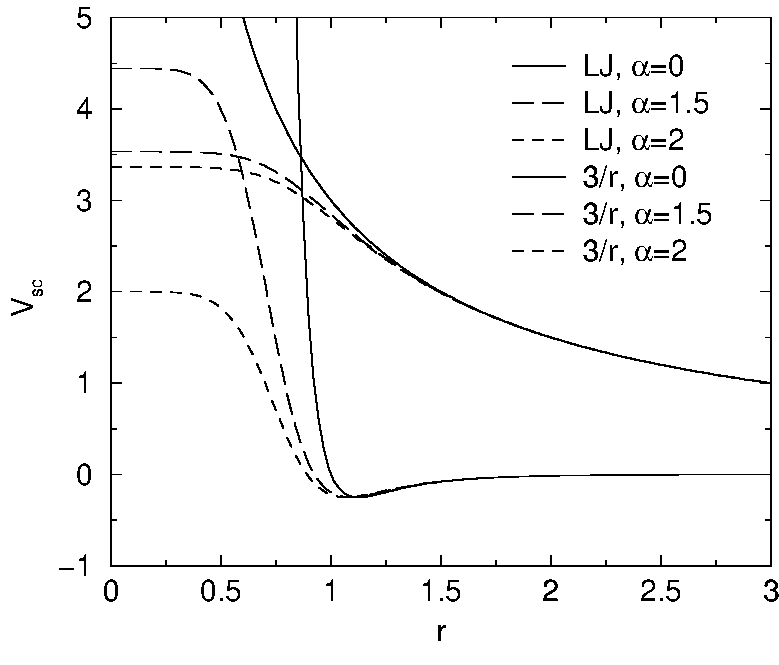
\includegraphics[height=6cm]{plots/softcore}}
\caption{Soft-core interactions at $\LAM=0.5$, with
$C_6^A=C_{12}^A=C_6^B=C_{12}^B=1$.}
\label{fig:softcore}
\end{figure}
The linear interpolation of the Lennard-Jones and Coulomb potentials gives
problems when growing particles out of nothing or when making particles
disappear ($\LAM$ close to 0 or 1). To circumvent these problems, the
singularities in the potentials need to be removed. This is done with
soft-core potentials. In {\gromacs} the soft-core potential $V_{sc}$ is:
\beq
V_{sc}(r) = \LL V^A(r_A) + \LAM V^B(r_B)
\eeq
\beq
r_A = \left(\alpha \sigma_A^6 \LAM^2 + r^6 \right)^\frac{1}{6}
\eeq
\beq
r_B = \left(\alpha \sigma_B^6 \LL^2 + r^6 \right)^\frac{1}{6}
\eeq
where $V^A$ and $V^B$ are the normal ``hard core'' Van der Waals or
electrostatic potentials in state A ($\LAM=0$) and state B ($\LAM=1$)
respectively, $\alpha$ is the soft-core parameter, which mainly controls the
height of the potential around $r=0$, $\sigma$ is the radius of the
interaction, which is $(C_{12}/C_6)^{1/6}$ or a predefined value when
$C_6$ or $C_{12}$ is zero.
For intermediate $\LAM$, $r_A$ and $r_B$ alter the interactions very little
when $r > \alpha^{1/6} \sigma$ and they quickly switch the soft-core
interaction to an almost constant value when $r$ becomes smaller
(\figref{softcore}). 
The force is:
\beq
F_{sc}(r) = -\frac{\partial V_{sc}(r)}{\partial r} =
 \LL F^A(r_A) \left(\frac{r}{r_A}\right)^5 +
\LAM F^B(r_B) \left(\frac{r}{r_B}\right)^5
\eeq
where $F^A$ and $F^B$ are the 'hard core' forces.
The contribution to the derivative of the free energy is:
\beq
\dvdl{V_{sc}(r)} =
-V^A(r_A) + V^B(r_B) +
\frac{1}{3} \alpha \LAM \LL 
\left( -F^A(r_A) \sigma_A^6 r_A^{-5} + F^B(r_B) \sigma_B^6 r_B^{-5} \right)
\eeq

\section{Methods}
\subsection{Exclusions and 1-4 Interactions.}
Atoms within a molecule that are close by in the chain, 
{\ie} atoms that are covalently bonded, or linked by one respectively two
atoms are so-called {\em first neighbors, second neighbors} and 
{\em \swapindex{third}{neighbor}s}, (see \figref{chain}). Since the
interactions of atom {\bf i} with atoms {\bf i+1} and {\bf i+2} 

\begin{figure}
\centerline{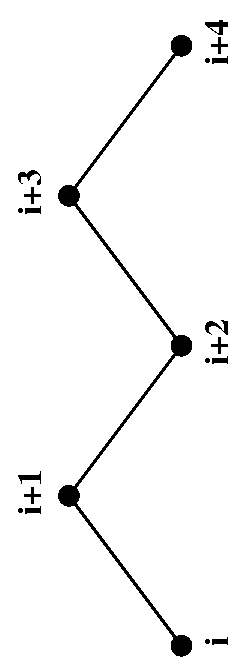
\includegraphics[angle=270,width=8cm]{plots/chain}}
\caption{Atoms along an alkane chain.}
\label{fig:chain}
\end{figure}

are mainly
quantum mechanical, they can not be modeled by a Lennard-Jones potential.
Instead it is assumed that these interactions are adequately modeled
by a harmonic bond term or constraint ({\bf i, i+1}) and a harmonic angle term
({\bf i, i+2}). The first and second neighbors (atoms {\bf i+1} and {\bf i+2}) 
are therefore
{\em excluded} from the Lennard-Jones \swapindex{interaction}{list} 
of atom {\bf i};
atoms {\bf i+1} and {\bf i+2} are called {\em \normindex{exclusions}} of atom {\bf i}.

For third neighbors the normal Lennard-Jones repulsion is sometimes
still too strong, which means that when applied to a molecule the
molecule would deform or break due to the internal strain. This is
especially the case for carbon-carbon interactions in a {\em
cis}-conformation ({\eg} {\em cis}-butane).  Therefore for some of these
interactions the Lennard-Jones repulsion has been reduced in the
{\gromos} force field, which is implemented by keeping a separate list of
1-4 and normal Lennard-Jones parameters. In other force fields, such
as OPLS~\cite{Jorgensen88}, the standard Lennard-Jones parameters are reduced
by a factor of two, but in that case also the dispersion (r$^{-6}$)
and the coulomb interaction are scaled.
{\gromacs} can use either of these methods.

\subsection{\normindex{Charge Group}s.}
\label{sec:cg}
In principle the force calculation in MD is an $O(N^2)$ problem.
Therefore we apply a \normindex{cutoff} for non-bonded force (NBF)
calculations: only the particles within a certain distance of each
other are interacting. This reduces the cost to $O(N)$ (typically
$100N$ to $200N$) of the NBF. It also introduces an error, which is,
in most cases, acceptable, except when applying the cutoff implies
the creation of charges, in which case you should consider using the
lattice sum methods provided by {\gromacs}.

Consider a water molecule interacting with another atom. When we would apply
the cutoff on an atom-atom basis we might include the atom-Oxygen
interaction (with a charge of -0.82) without the compensating charge
of the protons and so induce a large dipole moment over the system.
Therefore we have to keep groups of atoms with total charge
0 together. These groups are called {\em charge groups}.

\subsection{Treatment of cutoffs}
\newcommand{\rs}{$r_{short}$}
\newcommand{\rl}{$r_{long}$}
{\gromacs} is quite flexible in treating cutoffs, which implies
there can be quite a number of parameters to set. These parameters are
set in the input file for grompp. There are two sort of parameters
that affect the cutoff interactions; you can select which type
of interaction to use in each case, and which cutoffs should be
used in the neighborsearching.

For both Coulomb and van der Waals interactions there are interaction
type selectors
(termed {\tt vdwtype} and {\tt coulombtype}) and two parameters,
for a total of six nonbonded interaction parameters. See \secref{mdpopt} for a complete
description of these parameters.

The neighbor searching (NS) can be performed using a single-range, or a twin-range 
approach. Since the former is merely a special case of the latter we will 
discuss the more general twin-range. In this case NS is described by two
radii {\tt rlist} and max({\tt rcoulomb},{\tt rvdw}).
Usually one builds the neighbor list every 10 time steps
or every 20 fs (parameter {\tt nstlist}). In the neighbor list all interaction 
pairs that  fall within {\tt rlist} are stored. Furthermore, the 
interactions between pairs that do not
fall within {\tt rlist} but do fall within max({\tt rcoulomb},{\tt rvdw})
are computed during NS, and the
forces and energy are stored separately, and added to short-range forces
at every time step between successive NS. If {\tt rlist} = 
max({\tt rcoulomb},{\tt rvdw}), no forces
are evaluated during neighbor list generation.
The \normindex{virial} is calculated from the sum of the short- and
long-range forces.
This means that the virial can be slightly asymmetrical at non-NS steps.
In single precision the virial is almost always asymmetrical, because the
off-diagonal elements are about as large as each element in the sum.
In most cases this is not really a problem, since the fluctuations in de
virial can be 2 orders of magnitude larger than the average.

Except for the plain cutoff,
all of the interaction functions in \tabref{funcparm}
require that neighbor searching is done with a larger radius than the $r_c$
specified for the functional form, because of the use of charge groups.
The extra radius is typically of the order of 0.25 nm (roughly the 
largest distance between two atoms in a charge group plus the distance a 
charge group can diffuse within neighbor list updates).

%If your charge groups are very large it may be interesting to turn off charge
%groups, by setting the option 
%{\tt bAtomList = yes} in your {\tt grompp.mdp} file.
%In this case only a small extra radius to account for diffusion needs to be 
%added (0.1 nm). Do not however use this together with the plain cutoff
%method, as it will generate large artifacts (\secref{cg}).
%In summary, there are four parameters that describe NS behavior:
%{\tt nstlist} (update frequency in number of time steps),
%{\tt bAtomList} (whether or not charge groups are used to generate neighbor list, the default is to use charge groups, so {\tt bAtomList = no}),
%{\tt rshort} and {\tt rlong} which are the two radii {\rs} and {\rl}
%described above.

\begin{table}[ht]
\centering
\begin{tabular}{|ll|l|}
\dline
\multicolumn{2}{|c|}{Type}              & Parameters            \\
\hline
Coulomb&Plain cutoff   & $r_c$, $\epsr$        \\
&Reaction field         & $r_c$, $\epsrf$       \\
&Shift function         & $r_1$, $r_c$, $\epsr$         \\
&Switch function        & $r_1$, $r_c$, $\epsr$         \\
\hline
VdW&Plain cutoff       & $r_c$         \\
&Shift function         & $r_1$, $r_c$          \\
&Switch function        & $r_1$, $r_c$          \\
\dline
\end{tabular}
\caption[Parameters for the different functional forms of the
non-bonded interactions.]{Parameters for the different functional
forms of the non-bonded interactions.}
\label{tab:funcparm}
\end{table}


\newcommand{\Fi}{\ve{F}_i'}
\newcommand{\Fj}{\ve{F}_j'}
\newcommand{\Fk}{\ve{F}_k'}
\newcommand{\Fl}{\ve{F}_l'}
\newcommand{\Fvis}{\ve{F}_{d}}
\newcommand{\rvik}{\ve{r}_{ik}}
\newcommand{\rvid}{\ve{r}_{id}}
\newcommand{\rvjk}{\ve{r}_{jk}}
\newcommand{\rvjl}{\ve{r}_{jl}}

\section{Virtual interaction-sites}
\label{sec:virtual_sites}
\index{virtual interaction-sites}
Virtual interaction-sites (called \seeindex{dummy atoms}{virtual interaction-sites} in {\gromacs} versions before 3.3)
can be used in {\gromacs} in a number of ways. 
We write the position of the virtual site $\ve{r}_v$ as a function of
the positions of other particles \ve{r}$_i$: $\ve{r}_d =
f(\ve{r}_1..\ve{r}_n)$. The virtual site, which may carry charge, or can be
involved in other interactions can now be used in the force
calculation.  The force acting on the virtual site must be
redistributed over the particles with mass in a consistent way.
A good way to do this can be found in ref.~\cite{Berendsen84b}.
We can write the potential energy as
\beq
V = V(\ve{r}_v,\ve{r}_1..\ve{r}_n) = V^*(\ve{r}_1..\ve{r}_n)
\eeq
The force on the particle $i$ is then
\beq
\ve{F}_i = -\frac{\partial V^*}{\partial \ve{r}_i} 
         = -\frac{\partial V}{\partial \ve{r}_i} - 
            \frac{\partial \ve{r}_v}{\partial \ve{r}_i}
            \frac{\partial V}{\partial \ve{r}_v} 
         = \ve{F}_i^{direct} + \Fi
\eeq
the first term of which is the normal force. 
The second term is the force on particle $i$ due to the virtual site, which
can be written in tensor notation:
\newcommand{\partd}[2]{\displaystyle\frac{\partial #1}{\partial #2_i}}
\beq
\Fi = \left[\begin{array}{ccc}
\partd{x_v}{x} & \partd{y_v}{x} & \partd{z_v}{x}        \\[1ex]
\partd{x_v}{y} & \partd{y_v}{y} & \partd{z_v}{y}        \\[1ex]
\partd{x_v}{z} & \partd{y_v}{z} & \partd{z_v}{z}
\end{array}\right]\Fvis
\label{eqn:fvsite}
\eeq
where $\Fvis$ is the force on the virtual site and $x_v$, $y_v$ and
$z_v$ are the coordinates of the virtual site. In this way the total
force and the total torque are conserved~\cite{Berendsen84b}.

As a further note, the computation of the \normindex{virial}
(\eqnref{Xi}) is non-trivial when virtual sites are used. Since the
virial involves a summation over all the atoms (rather than virtual
sites) the forces most be redistributed from the virtual sites to the
atoms (using ~\eqnref{fvsite}) {\em before} computation of the
virial. In some special cases where the forces on the atoms can be
written as a linear combination of the forces on the virtual sites (types 2
and 3 below) there is no difference between computing the virial
before and after the redistribution of forces.  However, in the
general case redistribution should be done first.

\begin{figure}
\centerline{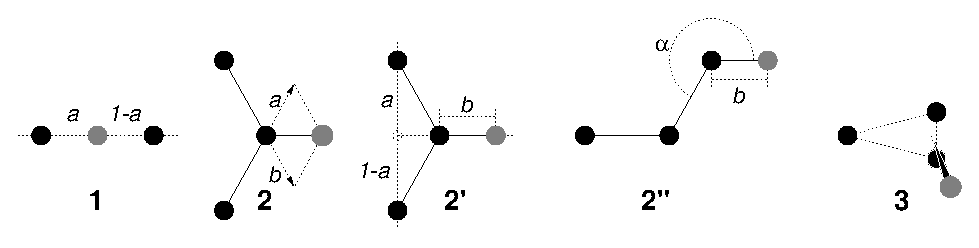
\includegraphics[width=15cm]{plots/dummies}}
\caption[Virtual site construction.]{The six different types of virtual
site construction in \protect{\gromacs}. The constructing atoms are
shown as black circles, the virutal sites in grey.}
\label{fig:vsites}
\end{figure}

There are six ways to construct virtual sites from surrounding atoms in
{\gromacs}, which we classify by the number of constructing
atoms. Note that all site types mentioned can be constructed from
types 3fd (normalized, in-plane) and 3out (non-normalized, out of
plane). However, the amount of computation involved increases sharply
along this list, so we strongly recommended using the first adequate
virtual site type that will be sufficient for a certain purpose.
\figref{vsites} gives an overview of the available virtual site constructions.

\begin{itemize}
\item[{\bf\sf 2.}]As a linear combination of two atoms
        (\figref{vsites} 2):
\beq
        \ve{r}_v ~=~ \ve{r}_i + a \rvij
\eeq
        In this case the virtual site is on the line through atoms $i$ and
        $j$. The force on particles $i$ and $j$ due to the force on
        the virtual site can be computed as:
\beq
        \begin{array}{lcr}
        \Fi &=& (1-a)\Fvis      \\
        \Fj &=& a\,\Fvis        \\
        \end{array}
\eeq

\item[{\bf\sf 3.}]As a linear combination of three atoms
        (\figref{vsites} 3):
\beq
        \ve{r}_v ~=~ \ve{r}_i + a \rvij + b \rvik
\eeq
        In this case the virtual site is in the plane of the other three
	particles.
        The force on particles $i$, $j$ and $k$ due to the force on the virtual
        site can be computed as:
\beq
        \begin{array}{lcr}
        \Fi &=& (1-a-b)\Fvis    \\
        \Fj &=& a\,\Fvis        \\
        \Fk &=& b\,\Fvis        \\
        \end{array}
\eeq

\item[{\bf\sf 3fd.}]In the plane of three atoms, with a fixed distance
        (\figref{vsites} 3fd):
\beq
        \ve{r}_v ~=~ \ve{r}_i + b \frac{  \rvij + a \rvjk  }
                                     {| \rvij + a \rvjk |}      
\eeq
        In this case the virtual site is in the plane of the other three
        particles at a distance of $|b|$ from $i$.
        The force on particles $i$, $j$ and $k$ due to the force on the virtual
        site can be computed as:
\beq
        \begin{array}{lcr}
        \Fi &=& \displaystyle \Fvis - \gamma ( \Fvis - \ve{p} ) \\[1ex]
        \Fj &=& \displaystyle (1-a)\gamma (\Fvis - \ve{p})      \\[1ex]
        \Fk &=& \displaystyle a \gamma (\Fvis - \ve{p})         \\
        \end{array}
        ~\mbox{~ where~ }~
        \begin{array}{c}
\displaystyle \gamma = \frac{b}{| \rvij + a \rvjk |} \\[2ex]
\displaystyle \ve{p} = \frac{ \rvid \cdot \Fvis }
                      { \rvid \cdot \rvid } \rvid
        \end{array}
\eeq

\item[{\bf\sf 3fad.}]In the plane of three atoms, with a fixed angle and
        distance (\figref{vsites} 3fad):
\beq
\label{eqn:vsite2fad-F}
         \ve{r}_v ~=~ \ve{r}_i +
                    d \cos \theta \frac{\rvij}{|\rvij|} +
                    d \sin \theta \frac{\ve{r}_\perp}{|\ve{r}_\perp|}
        ~\mbox{~ where~ }~
        \ve{r}_\perp ~=~ \rvjk - 
                        \frac{ \rvij \cdot \rvjk }
                             { \rvij \cdot \rvij }
                         \rvij
\eeq
        In this case the virtual site is in the plane of the other three
        particles at a distance of $|d|$ from $i$ at an angle of
        $\alpha$ with $\rvij$. Atom $k$ defines the plane and the
        direction of the angle. Note that in this case $b$ and
        $\alpha$ must be specified, instead of $a$ and $b$ (see also
        \secref{vsitetop}). The force on particles $i$, $j$ and $k$
        due to the force on the virtual site can be computed as (with
        $\ve{r}_\perp$ as defined in \eqnref{vsite2fad-F}):
\newcommand{\dfrac}{\displaystyle\frac}
\beq
\begin{array}{c}
        \begin{array}{lclllll}
        \Fi &=& \Fvis &-& 
                \dfrac{d \cos \theta}{|\rvij|} \ve{F}_1 &+&
                \dfrac{d \sin \theta}{|\ve{r}_\perp|} \left( 
                \dfrac{ \rvij \cdot \rvjk }
                     { \rvij \cdot \rvij } \ve{F}_2     +
                \ve{F}_3 \right)                                \\[3ex]
        \Fj &=& &&
                \dfrac{d \cos \theta}{|\rvij|} \ve{F}_1 &-&
                \dfrac{d \sin \theta}{|\ve{r}_\perp|} \left(
                 \ve{F}_2 + 
                 \dfrac{ \rvij \cdot \rvjk }
                        { \rvij \cdot \rvij } \ve{F}_2 +
                \ve{F}_3 \right)                                \\[3ex]
        \Fk &=& && &&
                \dfrac{d \sin \theta}{|\ve{r}_\perp|} \ve{F}_2  \\[3ex]
        \end{array}                                             \\[5ex]
        \mbox{where ~}
        \ve{F}_1 = \Fvis -
                  \dfrac{ \rvij \cdot \Fvis }
                        { \rvij \cdot \rvij } \rvij
        \mbox{\,, ~}
        \ve{F}_2 = \ve{F}_1 -
                  \dfrac{ \ve{r}_\perp \cdot \Fvis }
                        { \ve{r}_\perp \cdot \ve{r}_\perp } \ve{r}_\perp
        \mbox{~and ~}
        \ve{F}_3 = \dfrac{ \rvij \cdot \Fvis }
                         { \rvij \cdot \rvij } \ve{r}_\perp
\end{array}
\eeq

\item[{\bf\sf 3out.}]As a non-linear combination of three atoms, out of plane
        (\figref{vsites} 3out):
\beq
        \ve{r}_v ~=~ \ve{r}_i + a \rvij + b \rvik +
                c (\rvij \times \rvik)
\eeq
        This enables the construction of virtual sites out of the plane of the
        other atoms.
        The force on particles $i,j$ and $k$ due to the force on the virtual
        site can be computed as:
\beq
\begin{array}{lcl}
\vspace{4mm}
\Fj &=& \left[\begin{array}{ccc}
 a              &  -c\,z_{ik}   & c\,y_{ik}     \\[0.5ex]
 c\,z_{ik}      &   a           & -c\,x_{ik}    \\[0.5ex]
-c\,y_{ik}      &   c\,x_{ik}   & a
\end{array}\right]\Fvis                                 \\
\vspace{4mm}
\Fk &=& \left[\begin{array}{ccc}
 b              &   c\,z_{ij}   & -c\,y_{ij}    \\[0.5ex]
-c\,z_{ij}      &   b           & c\,x_{ij}     \\[0.5ex]
 c\,y_{ij}      &  -c\,x_{ij}   & b
\end{array}\right]\Fvis                                 \\
\Fi &=& \Fvis - \Fj - \Fk
\end{array}
\eeq

\item[{\bf\sf 4fd.}]From four atoms, with a fixed distance
        (\figref{vsites} 4fd):
\beq
        \ve{r}_v ~=~ \ve{r}_i + c \frac{  \rvij + a \rvjk + b \rvjl }
                                     {| \rvij + a \rvjk + b \rvjl|}     
\eeq
        In this case the virtual site is at a distance of $|c|$ from $i$.
        The force on particles $i$, $j$, $k$ and $l$ due to the force 
        on the virtual site can be computed as:
\beq
        \begin{array}{lcr}
        \Fi &=& \displaystyle \Fvis - \gamma ( \Fvis - \ve{p} ) \\[1ex]
        \Fj &=& \displaystyle (1-a-b)\gamma (\Fvis - \ve{p})    \\[1ex]
        \Fk &=& \displaystyle a \gamma (\Fvis - \ve{p})         \\[1ex]
        \Fl &=& \displaystyle b \gamma (\Fvis - \ve{p})         \\
        \end{array}
        ~\mbox{~ where~ }~
        \begin{array}{c}
\displaystyle \gamma = \frac{c}{| \rvij + a \rvjk + b \rvjl |} \\[2ex]
\displaystyle \ve{p} = \frac{ \rvid \cdot \Fvis }
                      { \rvid \cdot \rvid } \rvid
        \end{array}
\eeq


\end{itemize}

\newcommand{\dr}{{\rm d}r}
\newcommand{\avcsix}{\left< C_6 \right>}

\section{Dispersion correction}
\index{dispersion correction}
In this section we derive long range corrections due to the use of a
cut-off for Lennard Jones or Buckingham interactions.
We assume that the cut-off is
so long that the repulsion term can safely be neglected, and therefore
only the dispersion term is taken into account. Due to the nature of
the dispersion interaction, energy and pressure corrections both are
negative. While the energy correction is usually small, it may be
important for free energy calculations. The pressure correction in
contrast is very large and can not be neglected. Although it is in
principle possible to parameterize a force field such that the pressure
is close to 1 bar even without correction, such a method makes the
parameterization dependent on the cut-off and is therefore
undesirable. Please note that it is not consistent to use the long
range correction to the dispersion without using either a
\normindex{reaction field} method or a proper long range
electrostatics method such as Ewald summation or PPPM.

\subsection{Energy}
\label{sec:ecorr}
The long range contribution of the dispersion interaction to the
virial can be derived analytically, if we assume a homogeneous
system beyond the cut-off distance $r_c$. The dispersion energy
between two particles is written as:
\beq
V(\rij)	~=~	- C_6\,\rij^{-6}
\eeq
and the corresponding force is
\beq
\Fvij	~=~	- 6\,C_6\,\rij^{-8}\rvij
\eeq
In a periodic system it is not easy to calculate the full potentials,
so usually a cut-off is applied, which can be abrupt or smooth.
We will call the potential and force with cut-off $V_c$ and $\ve{F}_c$.
The long-range contribution to the dispersion energy
in a system with $N$ particles and particle density $\rho$ = $N/V$ is:
\beq
\label{eqn:enercorr}
V_{lr}  ~=~ \half N \rho\int_0^{\infty}   4\pi r^2 g(r) \left( V(r) -V_c(r) \right) {\dr}
\eeq
We will integrate this for the shift function, which is the most general
form of Van der Waals interaction available in Gromacs.
The shift function has a constant difference $S$ from 0 to $r_1$
and is 0 beyond the cut-off distance $r_c$.
We can integrate \eqnref{enercorr} assuming that the density in the sphere
within $r_1$ is equal to the global density and
the radial distribution function $g(r)$ is 1 beyond $r_1$:
\bea
\nonumber
V_{lr}  &=& \half N \left(
  \rho\int_0^{r_1}  4\pi r^2 g(r) \, C_6 \,S\,{\dr}
+ \rho\int_{r_1}^{r_c}  4\pi r^2 \left( V(r) -V_c(r) \right) {\dr}
+ \rho\int_{r_c}^{\infty}  4\pi r^2 V(r) \, {\dr}
\right) \\
& = & \half N \left(\left(\frac{4}{3}\pi \rho r_1^{3} - 1\right) C_6 \,S
+ \rho\int_{r_1}^{r_c} 4\pi r^2 \left( V(r) -V_c(r) \right) {\dr}
-\frac{4}{3} \pi N \rho\, C_6\,r_c^{-3}
\right)
\eea
where the term $-1$ corrects for the self-interaction.
For a plain cut-off we only need to assume that $g(r)$ is 1 beyond $r_c$
and the correction reduces to~\cite{Allen87}:
\bea
V_{lr} & = & -\frac{2}{3} \pi N \rho\, C_6\,r_c^{-3}
\eea
If we consider for example a box of pure water, simulated with a cut-off
of 0.9 nm and a density of 1 g cm$^{-3}$ this correction is 
-0.75 kJ mol$^{-1}$ per molecule.

For a homogeneous mixture we need to define 
an {\em average dispersion constant}:
\beq
\label{eqn:avcsix}
\avcsix	= \frac{2}{N(N-1)}\sum_i^N\sum_{j>i}^N C_6(i,j)\\
\eeq
In {\gromacs} excluded pairs of atoms do not contribute to the average.

In the case of inhomogeneous simulation systems, {\eg} a system with a
lipid interface, the energy correction can be applied if 
$\avcsix$ for both components is comparable.

\subsection{Virial and pressure}
The scalar virial of the system due to the dispersion interaction between
two particles $i$ and $j$ is given by:
\beq
\Xi	~=~	-\half \rvij \cdot \Fvij ~=~	3\,C_6\,\rij^{-6}
\eeq
The pressure is given by:
\beq
P	~=~	\frac{2}{3\,V}\left(E_{kin} - \Xi\right)
\eeq
The long-range correction to the virial is given by:
\beq
\Xi_{lr} ~=~ \half N \rho \int_0^{\infty} 4\pi r^2 g(r) (\Xi -\Xi_c) \,\dr
\eeq
We can again integrate the long range contribution to the 
virial assuming $g(r)$ is 1 beyond $r_1$:
\bea
\Xi_{lr}&=&	\half N \rho \left(
    \int_{r_1}^{r_c}  4 \pi r^2 (\Xi -\Xi_c)  \,\dr
  + \int_{r_c}^{\infty} 4 \pi r^2 3\,C_6\,\rij^{-6}\,  \dr
\right)	\nonumber\\
        &=&     \half N \rho \left(
    \int_{r_1}^{r_c} 4 \pi r^2 (\Xi -\Xi_c) \, \dr
  + 4 \pi C_6 \, r_c^{-3} \right)
\eea
For a plain cut-off the correction to the pressure is~\cite{Allen87}:
\beq
P_{lr}	~=~	-\frac{4}{3} \pi C_6\, \rho^2 r_c^{-3}
\eeq
Using the same example of a water box, the correction to the virial is
0.75 kJ mol$^{-1}$ per molecule,
the corresponding correction to the pressure for 
SPC water is approximately -280 bar.

For homogeneous mixtures we can again use the average dispersion constant
$\avcsix$ (\eqnref{avcsix}):
\beq
P_{lr}	~=~	-\frac{4}{3} \pi \avcsix \rho^2 r_c^{-3}
\label{eqn:pcorr}
\eeq
For inhomogeneous systems \eqnref{pcorr} can be applied under the same
restriction as holds for the energy (see \secref{ecorr}).


\section{Long Range Electrostatics}
\label{sec:lr_elstat}
\subsection{\normindex{Ewald sum}mation}
\label{sec:ewald}
The total electrostatic energy of $N$ particles and the periodic
images\index{periodic boundary conditions} are given by
\begin{equation}
V=\frac{f}{2}\sum_{n_x}\sum_{n_y}
\sum_{n_{z}*} \sum_{i}^{N} \sum_{j}^{N} 
\frac{q_i q_j}{{\bf r}_{ij,{\bf n}}}.
\label{eqn:totalcoulomb}
\end{equation}
$(n_x,n_y,n_z)={\bf n}$ is the box index vector, and the star indicates that
terms with $i=j$ should be omitted when $(n_x,n_y,n_z)=(0,0,0)$. The
distance ${\bf r}_{ij,{\bf n}}$ is the real distance between the charges and
not the minimum-image. This sum is conditionally convergent, but 
very slow.

Ewald summation was first introduced as a method to calculate
long-range interactions of the periodic images in
crystals~\cite{Ewald21}. The idea is to convert the single
slowly-converging sum \eqnref{totalcoulomb} into two
quickly-converging terms and a constant term:
\begin{eqnarray}
V &=& V_{dir} + V_{rec} + V_{0} \\[0.5ex]
V_{dir} &=& \frac{f}{2} \sum_{i,j}^{N} 
\sum_{n_x}\sum_{n_y}
\sum_{n_{z}*} q_i q_j \frac{\mbox{erfc}(\beta {r}_{ij,{\bf n}} )}{{r}_{ij,{\bf n}}} \\[0.5ex]
V_{rec} &=& \frac{f}{2 \pi V} \sum_{i,j}^{N} q_i q_j 
\sum_{m_x}\sum_{m_y}
\sum_{m_{z}*} \frac{\exp{\left( -(\pi {\bf m}/\beta)^2 + 2 \pi i
      {\bf m} \cdot ({\bf r}_i - {\bf r}_j)\right)}}{{\bf m}^2} \\[0.5ex]
V_{0} &=& -\frac{f \beta}{\sqrt{\pi}}\sum_{i}^{N} q_i^2,
\end{eqnarray}
where $\beta$ is a parameter that determines the relative weight of the
direct and reciprocal sums and ${\bf m}=(m_x,m_y,m_z)$.
In this way we can use a short cutoff (of the order of $1$~nm) in the direct space sum and a
short cutoff in the reciprocal space sum ({\eg} 10 wave vectors in each 
direction). Unfortunately, the computational cost of the reciprocal
part of the sum increases as $N^2$
(or $N^{3/2}$ with a slightly better algorithm) and it is therefore not 
realistic for use in large systems.

\subsubsection{Using Ewald}
Don't use Ewald unless you are absolutely sure this is what you want -
for almost all cases the PME method below will perform much better.
If you still want to employ classical Ewald summation enter this in
your {\tt .mdp} file, if the side of your box is about $3$~nm:
\begin{verbatim}
coulombtype     = Ewald
rvdw            = 0.9
rlist           = 0.9
rcoulomb        = 0.9
fourierspacing  = 0.6
ewald_rtol      = 1e-5
\end{verbatim}
The {\tt fourierspacing} parameter times the box dimensions determines
the highest magnitude of wave vectors $m_x,m_y,m_z$ to use in each
direction. With a 3~nm cubic box this example would use $11$ wave vectors
(from $-5$ to $5$) in each direction.  The {\tt ewald\_rtol} parameter
is the relative strength of the electrostatic interaction at the
cutoff. Decreasing this gives you a more accurate direct sum, but a
less accurate reciprocal sum.
 
\subsection{\normindex{PME}}
\label{sec:pme}
Particle-mesh Ewald is a method proposed by Tom
Darden~\cite{Darden93,Essmann95} to improve the performance of the
reciprocal sum. Instead of directly summing wave vectors, the charges
are assigned to a grid using cardinal B-spline interpolation. This
grid is then Fourier transformed with a 3D FFT algorithm and the
reciprocal energy term obtained by a single sum over the grid in
k-space.

The potential at the grid points is calculated by inverse
transformation, and by using the interpolation factors we get the
forces on each atom. 

The PME algorithm scales as $N \log(N)$, and is substantially faster
than ordinary Ewald summation on medium to large systems. On very
small systems it might still be better to use Ewald to avoid the
overhead in setting up grids and transforms.

\subsubsection{Using PME}
To use Particle-mesh Ewald summation in {\gromacs}, specify the
following lines in your {\tt .mdp} file:
\begin{verbatim}
coulombtype     = PME
rvdw            = 0.9
rlist           = 0.9
rcoulomb        = 0.9
fourierspacing  = 0.12
pme_order       = 4
ewald_rtol      = 1e-5
\end{verbatim}
In this case the {\tt fourierspacing} parameter determines the maximum
spacing for the FFT grid and {\tt pme\_order} controls the
interpolation order. Using 4th order (cubic) interpolation and this
spacing should give electrostatic energies accurate to about
$5\cdot10^{-3}$. Since the Lennard-Jones energies are not this
accurate it might even be possible to increase this spacing slightly.

Pressure scaling works with PME, but be aware of the fact that
anisotropic scaling can introduce artificial ordering in some systems.

\subsection{\normindex{PPPM}}
\label{sec:pppm}
The \seeindex{Particle-Particle Particle-Mesh}{PPPM} methods of
Hockney \& Eastwood can also be applied in {\gromacs} for the
treatment of long range electrostatic
interactions~\cite{Hockney81,Darden93,Luty95a}.  With this algorithm
the charges of all particles are spread over a grid of dimensions
($n_x$,$n_y$,$n_z$) using a weighting function called the
triangle-shaped charged distribution:
\beq
\begin{array}{lcl}
W(\ve{r}) &=&   W(x)~W(y)~W(z)  \\[1ex]
W(\xi)  &=& \left\{
\begin{array}{ll}
\frac{3}{4} - \left(\frac{\xi}{h}\right)^2 
        & |\xi| \leq \frac{h}{2}                                \\[0.5ex]
\frac{1}{2}\left(\frac{3}{2} - \frac{|\xi|}{h}\right)^2 
        & \frac{h}{2} < |\xi| < \frac{3h}{2}                    \\[0.5ex]
0       & \frac{3h}{2} \leq |\xi|                               \\[0.5ex]
\end{array}
\right.
\end{array}
\eeq
where $\xi$ (is x, y or z) is the distance to a grid point in the corresponding
dimension. Only the 27 closest grid points need to be taken into account for each charge.

Then, this charge distribution is Fourier transformed using a 3D inverse FFT 
routine.
In Fourier space a convolution with function $\hat{G}$ is performed:
\beq
\hat{G}(k)      ~=~     \frac{\hat{g}(k)}{\epsilon_0 k^2}
\eeq
where $\hat{g}$ is the Fourier transform of the charge spread function
g(r). This yield the long range potential $\hat{\phi}(k)$ on the mesh, which
can be transformed using a forward FFT routine into the real space potential.
Finally the potential and forces are retrieved using interpolation~\cite{Luty95a}.
%
% note - this accuracy is just a rough estimate...
%
It is not easy to calculate the full long-range virial tensor with
PPPM, but it is possible to obtain the trace. This means that the sum
of the pressure components is correct (and therefore the isotropic
pressure) but not necessarily the individual pressure components!

\subsubsection{Using PPPM}
To use the PPPM algorithm in {\gromacs}, specify the
following lines in your {\tt .mdp} file:
\begin{verbatim}
coulombtype     = PPPM
rlist           = 1.0
rcoulomb        = 0.85
rcoulomb_switch = 0.0
rvdw            = 1.0
fourierspacing  = 0.075
\end{verbatim}
For details on the switch parameters see the section on modified
long-range interactions in this manual. When using PPPM we recommend
to take at most 0.075 nm per gridpoint ({\eg} 20 gridpoints for 1.5
nm).  PPPM does not provide the same accuracy as PME but can be
slightly faster in some cases. Due to the problem with the pressure
tensor you shouldn't use it with pressure coupling.

We're somewhat ambivalent about PPPM, so if you use it please contact
us - otherwise it might be removed from future relases so we can concentrate
our efforts on PME.


\subsection{Optimizing Fourier transforms}
To get the best possible performance you should try to avoid large
prime numbers for grid dimensions.
The FFT code used in {\gromacs} is
optimized for grid sizes of the form $2^a 3^b 5^c 7^d 11^e 13^f$,
where $e+f$ is $0$ or $1$ and the other exponents arbitrary. (See
further the documentation of the FFT algorithms at 
\href{http://www.fftw.org}{www.fftw.org}.

It is also possible to optimize the transforms for the current problem
by performing some calculations at the start of the run. This is not
done per default since it takes a couple of minutes, but for large
runs it will save time. Turn it on by specifying

\begin{verbatim}
optimize_fft      = yes
\end{verbatim}
in your {\tt .mdp} file.

When running in parallel the grid must be communicated several times
and thus hurting scaling performance. With PME you can improve this
by increasing grid spacing while simultaneously increasing the
interpolation to {\eg} 6th order. 
Since the interpolation is entirely local a this will
improve the scaling in most cases.

%
% Temporarily removed since I'm not sure about the state of the testlr 
% program...
%
%It is possible to test the accuracy of your settings using the program 
%{\tt\normindex{testlr}} in the {\tt src/gmxlib} dir. This program computes
%forces and potentials using PPPM and an Ewald implementation and gives the
%absolute and RMS errors in both:
%\begin{verbatim}
%ERROR ANALYSIS
%Error:         Max Abs         RMS            
%Force            1.132       0.251
%Potential        0.113       0.035
%\end{verbatim}
%{\bf Note:} these numbers were generated using a grid spacing of
%0.058 nm and $r_c$ = 1.0 nm.
%
%You can see what the accuracy is without optimizing the
%$\hat{G}(k)$ function, if you pass the {\tt -ghat} option to {\tt
%testlr}. Try it if you think the {\tt mk\_ghat} procedure is a waste
%of time.


\section{\swapindex{All-hydrogen}{force-field}}
The {\gromacs} all-hydrogen force-field is almost identical to the normal
{\gromacs} forcefield, since the extra hydrogens have no Lennard-Jones
interaction and zero charge. The only differences are in the bond angle
and improper dihedral angle terms. This forcefield is only useful when
you need the exact hydrogen positions, for instance for distance
restraints derived from NMR measurements.

\section{\gromosv{96} notes}

\subsection{The \gromosv{96} force field\index{gromos-96 force field}}
{\gromacs} supports the \gromosv{96} force fields~\cite{gromos96}.
All parameters for the 43a1, 43a2 (development, improved alkane
dihedrals) and 43b1 (vacuum) force fields are included.  All standard
building blocks are included and topologies can be build automatically
by {\tt pdb2gmx}.  The \gromosv{96} force field is a further
development of the \gromosv{87} force field on which the {\gromacs}
forcefield is based. The \gromosv{96} force field has improvements
over the {\gromacs} force field for proteins and small molecules.
It is not, however, recommended for use with long alkanes and
lipids.  The \gromosv{96} force field differs from the {\gromacs}
force field in a few aspects:
\begin{itemize}
\item the force field parameters
\item the parameters for the bonded interactions are not linked to atom types
\item a fourth power bond stretching potential (\secref{bondpot})
\item an angle potential based on the cosine of the angle (\secref{anglepot})
\end{itemize}
There are two differences in implementation between {\gromacs} and \gromosv{96}
which can lead to slightly different results when simulating the same system
with both packages: 
\begin{itemize}
\item in \gromosv{96} neighbor searching for solvents is performed on the
first atom of the solvent molecule, this is not implemented in {\gromacs},
but the difference with searching with centers of charge groups is very small
\item the virial in \gromosv{96} is molecule-based. This is not implemented in
{\gromacs}, which uses atomic virials
\end{itemize}
The \gromosv{96} force field was parameterized with a Lennard-Jones cutoff
of 1.4 nm, so be sure to use a Lennard-Jones cutoff of at least 1.4.
A larger cutoff is possible, because the Lennard-Jones potential and forces
are almost zero beyond 1.4 nm.

\subsection{\gromosv{96} files}\index{gromos-96 files}\index{files,
gromos|see{gromos-96 files}}
{\gromacs} can read and write \gromosv{96} coordinate and trajectory files.
These files should have the extension {\tt .g96}.
Such a file can be a \gromosv{96} initial/final
configuration file or a coordinate trajectory file or a combination of both.
The file is fixed format; all floats are written as 15.9 (files can get huge).
{\gromacs} supports the following data blocks in the given order:
\begin{itemize}
\item Header block:
\begin{verbatim}
TITLE (mandatory)
\end{verbatim}
\item Frame blocks:
\begin{verbatim}
TIMESTEP (optional)
POSITION/POSITIONRED (mandatory)
VELOCITY/VELOCITYRED (optional)
BOX (optional)
\end{verbatim}
\end{itemize}
See the \gromosv{96} manual~\cite{gromos96} for a complete description
of the blocks. Note that all {\gromacs} programs can read compressed
(.Z) or gzipped (.gz) files.
